% Options for packages loaded elsewhere
\PassOptionsToPackage{unicode}{hyperref}
\PassOptionsToPackage{hyphens}{url}
\PassOptionsToPackage{dvipsnames,svgnames,x11names}{xcolor}
%
\documentclass[
  ignorenonframetext,
  t]{beamer}
\usepackage{pgfpages}
\setbeamertemplate{caption}[numbered]
\setbeamertemplate{caption label separator}{: }
\setbeamercolor{caption name}{fg=normal text.fg}
\beamertemplatenavigationsymbolsempty
% Prevent slide breaks in the middle of a paragraph
\widowpenalties 1 10000
\raggedbottom
\setbeamertemplate{part page}{
  \centering
  \begin{beamercolorbox}[sep=16pt,center]{part title}
    \usebeamerfont{part title}\insertpart\par
  \end{beamercolorbox}
}
\setbeamertemplate{section page}{
  \centering
  \begin{beamercolorbox}[sep=12pt,center]{part title}
    \usebeamerfont{section title}\insertsection\par
  \end{beamercolorbox}
}
\setbeamertemplate{subsection page}{
  \centering
  \begin{beamercolorbox}[sep=8pt,center]{part title}
    \usebeamerfont{subsection title}\insertsubsection\par
  \end{beamercolorbox}
}
\AtBeginPart{
  \frame{\partpage}
}
\AtBeginSection{
  \ifbibliography
  \else
    \frame{\sectionpage}
  \fi
}
\AtBeginSubsection{
  \frame{\subsectionpage}
}

\usepackage{amsmath,amssymb}
\usepackage{iftex}
\ifPDFTeX
  \usepackage[T1]{fontenc}
  \usepackage[utf8]{inputenc}
  \usepackage{textcomp} % provide euro and other symbols
\else % if luatex or xetex
  \usepackage{unicode-math}
  \defaultfontfeatures{Scale=MatchLowercase}
  \defaultfontfeatures[\rmfamily]{Ligatures=TeX,Scale=1}
\fi
\usepackage{lmodern}
\usetheme[]{Singapore}
\usefonttheme{serif} % use mainfont rather than sansfont for slide text
\ifPDFTeX\else  
    % xetex/luatex font selection
    \setmainfont[]{Brill}
    \setmonofont[]{Iosevka}
\fi
% Use upquote if available, for straight quotes in verbatim environments
\IfFileExists{upquote.sty}{\usepackage{upquote}}{}
\IfFileExists{microtype.sty}{% use microtype if available
  \usepackage[]{microtype}
  \UseMicrotypeSet[protrusion]{basicmath} % disable protrusion for tt fonts
}{}
\makeatletter
\@ifundefined{KOMAClassName}{% if non-KOMA class
  \IfFileExists{parskip.sty}{%
    \usepackage{parskip}
  }{% else
    \setlength{\parindent}{0pt}
    \setlength{\parskip}{6pt plus 2pt minus 1pt}}
}{% if KOMA class
  \KOMAoptions{parskip=half}}
\makeatother
\usepackage{xcolor}
\newif\ifbibliography
\ifLuaTeX
  \usepackage{luacolor}
  \usepackage[soul]{lua-ul}
\else
  \usepackage{soul}
  \makeatletter
  \let\HL\hl
  \renewcommand\hl{% fix for beamer highlighting
    \let\set@color\beamerorig@set@color
    \let\reset@color\beamerorig@reset@color
    \HL}
  \makeatother
  
\fi
\setlength{\emergencystretch}{3em} % prevent overfull lines
\setcounter{secnumdepth}{-\maxdimen} % remove section numbering


\providecommand{\tightlist}{%
  \setlength{\itemsep}{0pt}\setlength{\parskip}{0pt}}\usepackage{longtable,booktabs,array}
\usepackage{calc} % for calculating minipage widths
\usepackage{caption}
% Make caption package work with longtable
\makeatletter
\def\fnum@table{\tablename~\thetable}
\makeatother
\usepackage{graphicx}
\makeatletter
\def\maxwidth{\ifdim\Gin@nat@width>\linewidth\linewidth\else\Gin@nat@width\fi}
\def\maxheight{\ifdim\Gin@nat@height>\textheight\textheight\else\Gin@nat@height\fi}
\makeatother
% Scale images if necessary, so that they will not overflow the page
% margins by default, and it is still possible to overwrite the defaults
% using explicit options in \includegraphics[width, height, ...]{}
\setkeys{Gin}{width=\maxwidth,height=\maxheight,keepaspectratio}
% Set default figure placement to htbp
\makeatletter
\def\fps@figure{htbp}
\makeatother

\setbeamertemplate{footline}[page number]
\usepackage{caption}
\captionsetup[figure]{labelformat=empty}
\captionsetup[subfigure]{labelformat=empty}
\setbeamercolor{alerted text}{fg=teal}
\makeatletter
\@ifpackageloaded{caption}{}{\usepackage{caption}}
\AtBeginDocument{%
\ifdefined\contentsname
  \renewcommand*\contentsname{Table of contents}
\else
  \newcommand\contentsname{Table of contents}
\fi
\ifdefined\listfigurename
  \renewcommand*\listfigurename{List of Figures}
\else
  \newcommand\listfigurename{List of Figures}
\fi
\ifdefined\listtablename
  \renewcommand*\listtablename{List of Tables}
\else
  \newcommand\listtablename{List of Tables}
\fi
\ifdefined\figurename
  \renewcommand*\figurename{Figure}
\else
  \newcommand\figurename{Figure}
\fi
\ifdefined\tablename
  \renewcommand*\tablename{Table}
\else
  \newcommand\tablename{Table}
\fi
}
\@ifpackageloaded{float}{}{\usepackage{float}}
\floatstyle{ruled}
\@ifundefined{c@chapter}{\newfloat{codelisting}{h}{lop}}{\newfloat{codelisting}{h}{lop}[chapter]}
\floatname{codelisting}{Listing}
\newcommand*\listoflistings{\listof{codelisting}{List of Listings}}
\makeatother
\makeatletter
\makeatother
\makeatletter
\@ifpackageloaded{caption}{}{\usepackage{caption}}
\@ifpackageloaded{subcaption}{}{\usepackage{subcaption}}
\makeatother

\ifLuaTeX
\usepackage[bidi=basic]{babel}
\else
\usepackage[bidi=default]{babel}
\fi
\babelprovide[main,import]{english}
\ifPDFTeX
\else
\babelfont{rm}[]{Brill}
\fi
% get rid of language-specific shorthands (see #6817):
\let\LanguageShortHands\languageshorthands
\def\languageshorthands#1{}
\ifLuaTeX
  \usepackage{selnolig}  % disable illegal ligatures
\fi
\usepackage[]{natbib}
\bibliographystyle{plainnat}
\usepackage{bookmark}

\IfFileExists{xurl.sty}{\usepackage{xurl}}{} % add URL line breaks if available
\urlstyle{same} % disable monospaced font for URLs
\hypersetup{
  pdftitle={The DiaL2 project: pipeline, results, news and future work},
  pdfauthor={George Moroz; Olga Gich; Anna Grishanova; Natalia Koshelyuk; Chiara Naccarato; Anna Panova; Anastasia Yakovleva; ; Svetlana Zemicheva},
  pdflang={en},
  colorlinks=true,
  linkcolor={Maroon},
  filecolor={Maroon},
  citecolor={teal},
  urlcolor={teal},
  pdfcreator={LaTeX via pandoc}}


\title{The DiaL2 project: pipeline, results, news and future work}
\author{George Moroz \and Olga Gich \and Anna Grishanova \and Natalia
Koshelyuk \and Chiara Naccarato \and Anna Panova \and Anastasia
Yakovleva \and  \and Svetlana Zemicheva}
\date{17.09.2024}

\begin{document}
\frame{\titlepage}
\begin{abstract}
There are 24 dialectal and 8 bilingual corpora of Russian at the
Linguistic Convergence Laboratory (see the resources page), and more are
coming. The DiaL2 project was launched two years ago with an aim to
study the linguistic variation found in these corpora. We applied a
UDpipe morphological and syntactic parser, manually annotated a set of
linguistic features (sometimes relistening the recordings in order to
check the transcriptions), and implemented statistical models for each
feature that predict the probability of divergence from Standard
Russian. During the talk we will discuss our results based on several
features:

\begin{itemize}
\tightlist
\item
  non-standard marking in numeral constructions (dva dom {[}two.M
  house.SG{]} `two houses');
\item
  preposition drop (rodilas' {[}v{]} tridcat' devjatom godu `(she) was
  born (in) nineteen thirty-nine');
\item
  non-standard marking in negative existential constructions (ranše
  sadiki ne byli `there were no kindergartens before.').
\end{itemize}

As possible predictors in the models, we used sociolinguistic features
(gender, year of birth, years of education), measures of
collocationality, and some relevant linguistic features. During the work
we discovered multiple typos, inconsistent and wrong transcriptions, and
corrected a lot of them. Therefore, we started a parallel project
dedicated to automatic correction of the Lab's corpora, which will also
be discussed during the talk.
\end{abstract}


\section{Precursors of the project}\label{precursors-of-the-project}

\begin{frame}{Precursors of the project}
\phantomsection\label{precursors-of-the-project-1}
\begin{figure}

\begin{minipage}{0.50\linewidth}

\begin{figure}[H]

{\centering 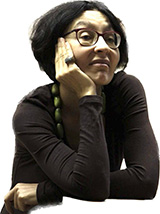
\includegraphics[width=0.53in,height=\textheight]{images/dobrushina.jpg}

}

\subcaption{Nina Dobrushina}

\end{figure}%

\end{minipage}%
%
\begin{minipage}{0.50\linewidth}

\begin{figure}[H]

{\centering 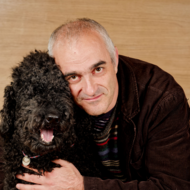
\includegraphics[width=0.63in,height=\textheight]{images/daniel.png}

}

\subcaption{Michael Daniel}

\end{figure}%

\end{minipage}%

\end{figure}%

\begin{itemize}
\tightlist
\item
  Multiple sociolinguistic expeditions to Daghestan
\item
  Several dialect expeditions to Ustya \pause
\item
  Online corpora available for everyone:

  \begin{itemize}
  \tightlist
  \item
    \href{https://parasolcorpus.org/dagrus/}{Corpus of Russian spoken in
    Daghestan}
  \item
    \href{https://www.parasolcorpus.org/Pushkino/login.php}{Ustja River
    Basin Corpus} \pause
  \item
    \ldots{} and other bilingual and dialect corpora
  \end{itemize}
\end{itemize}
\end{frame}

\begin{frame}{Resources of the Linguistic Convergence Laboratory}
\phantomsection\label{resources-of-the-linguistic-convergence-laboratory}
\begin{itemize}
\tightlist
\item
  \url{https://lingconlab.ru/}
\item
  24 dialectal corpora
\item
  8 bilingual corpora
\end{itemize}
\end{frame}

\begin{frame}{Dialectal Corpora}
\phantomsection\label{dialectal-corpora}
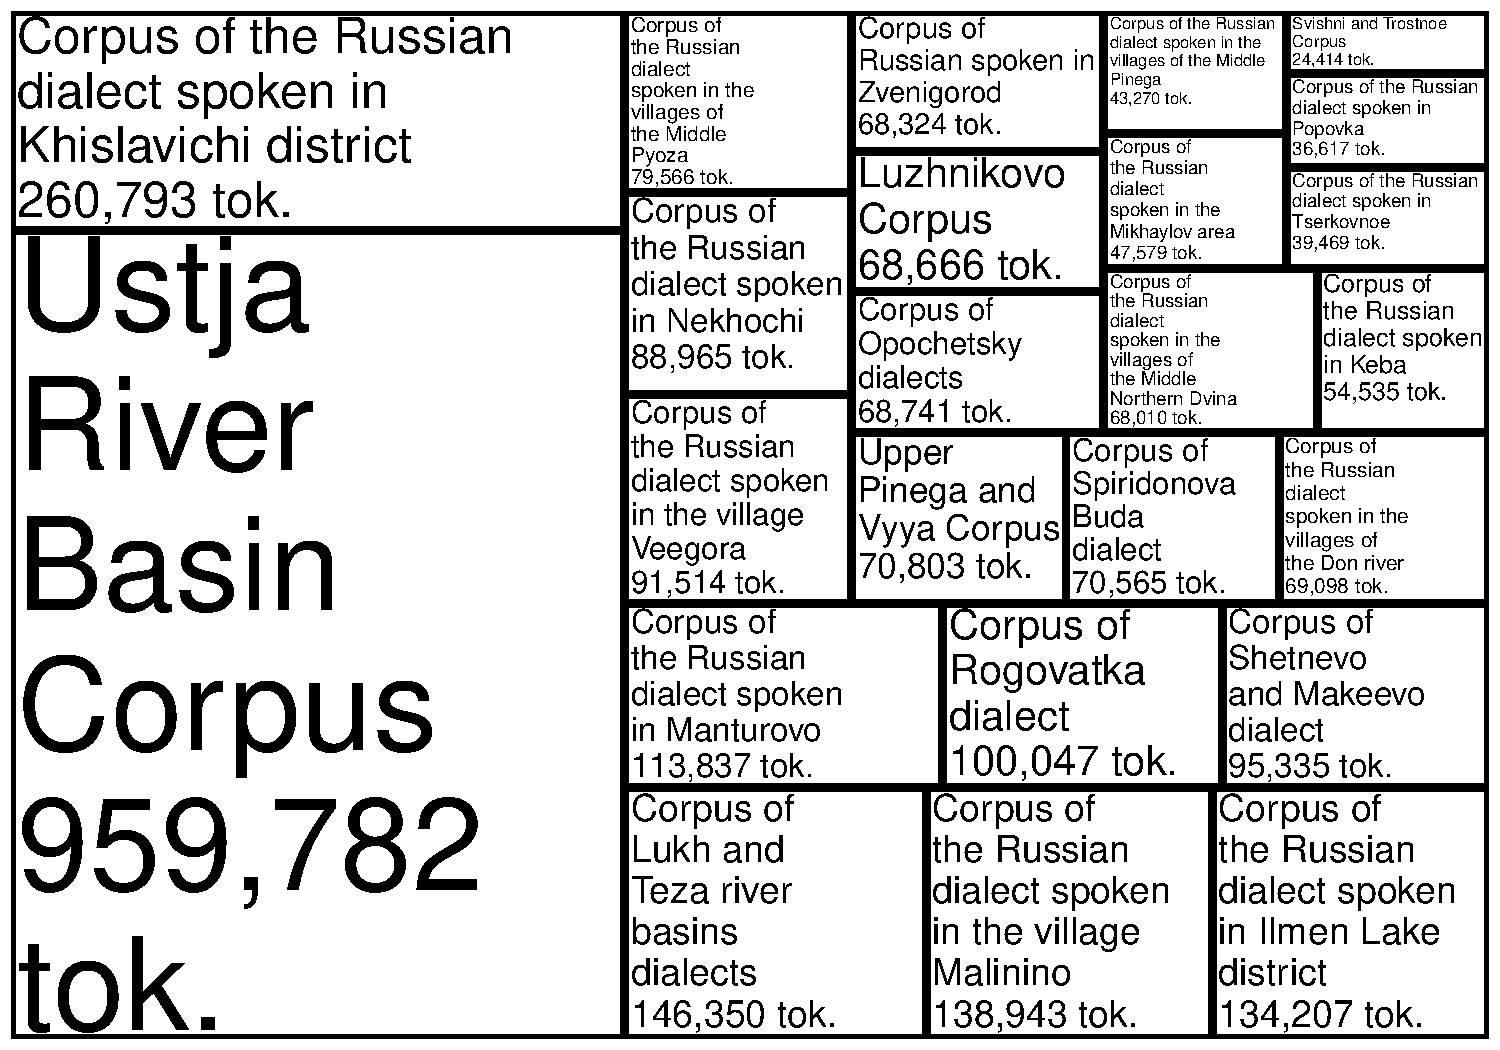
\includegraphics{2024.09.17_dial2_files/figure-beamer/unnamed-chunk-4-1.pdf}
\end{frame}

\begin{frame}{Bilingual Corpora}
\phantomsection\label{bilingual-corpora}
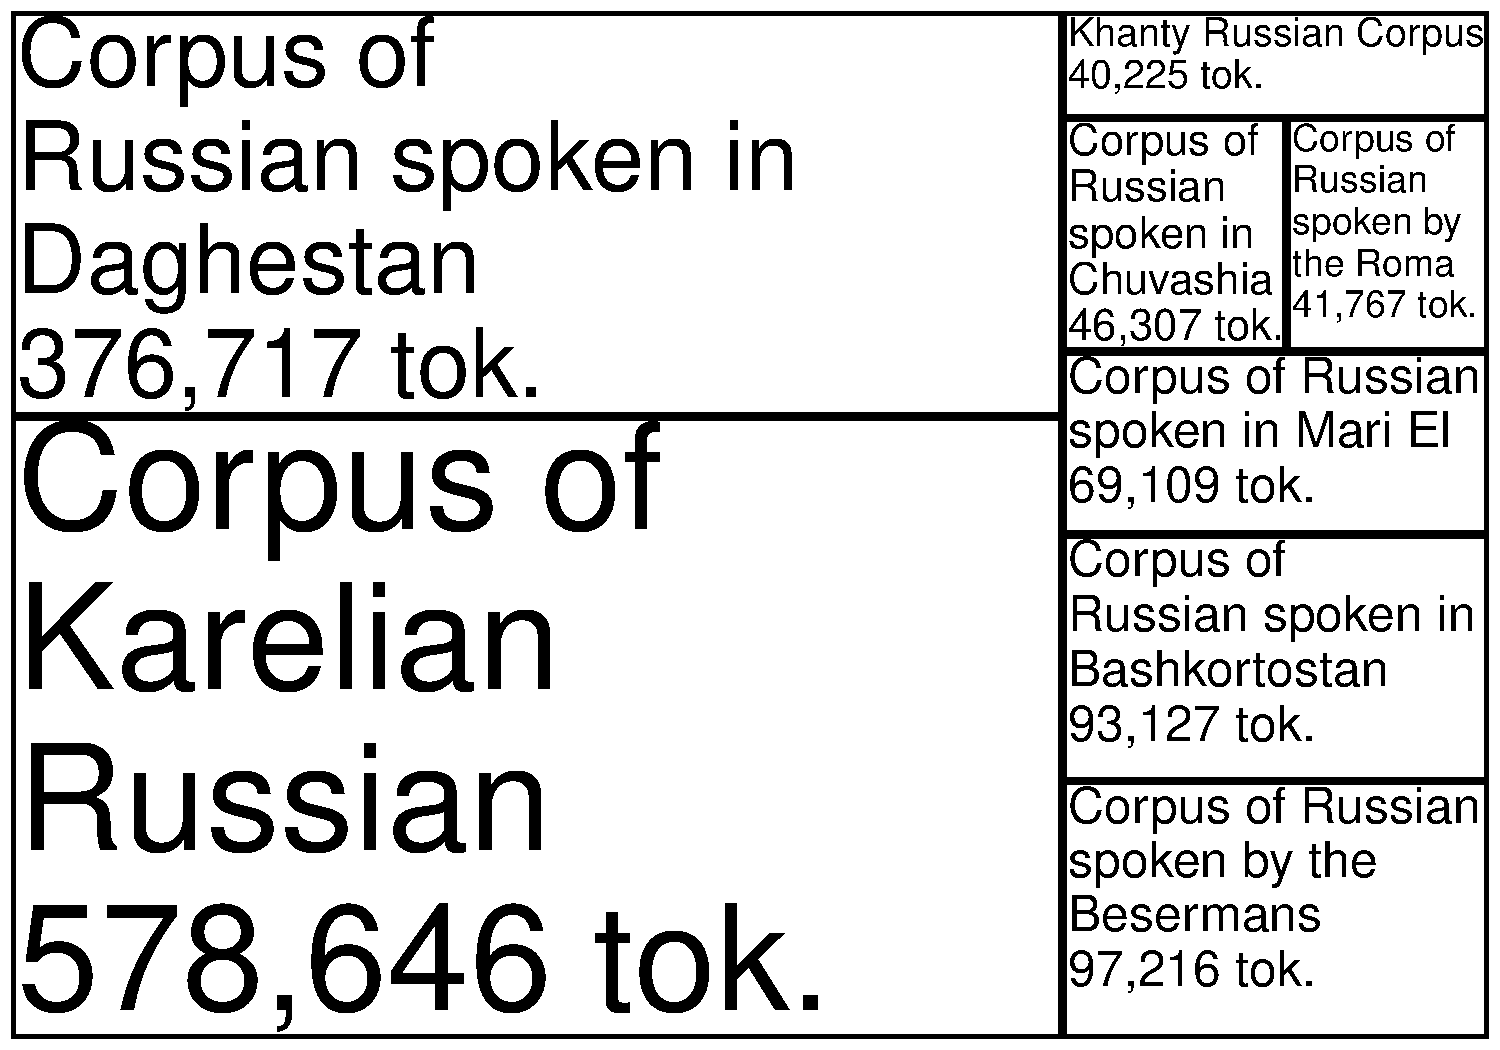
\includegraphics{2024.09.17_dial2_files/figure-beamer/unnamed-chunk-5-1.pdf}
\end{frame}

\begin{frame}[fragile]{Bilingual and Dialectal Corpora}
\phantomsection\label{bilingual-and-dialectal-corpora}
\begin{figure}[H]

{\centering 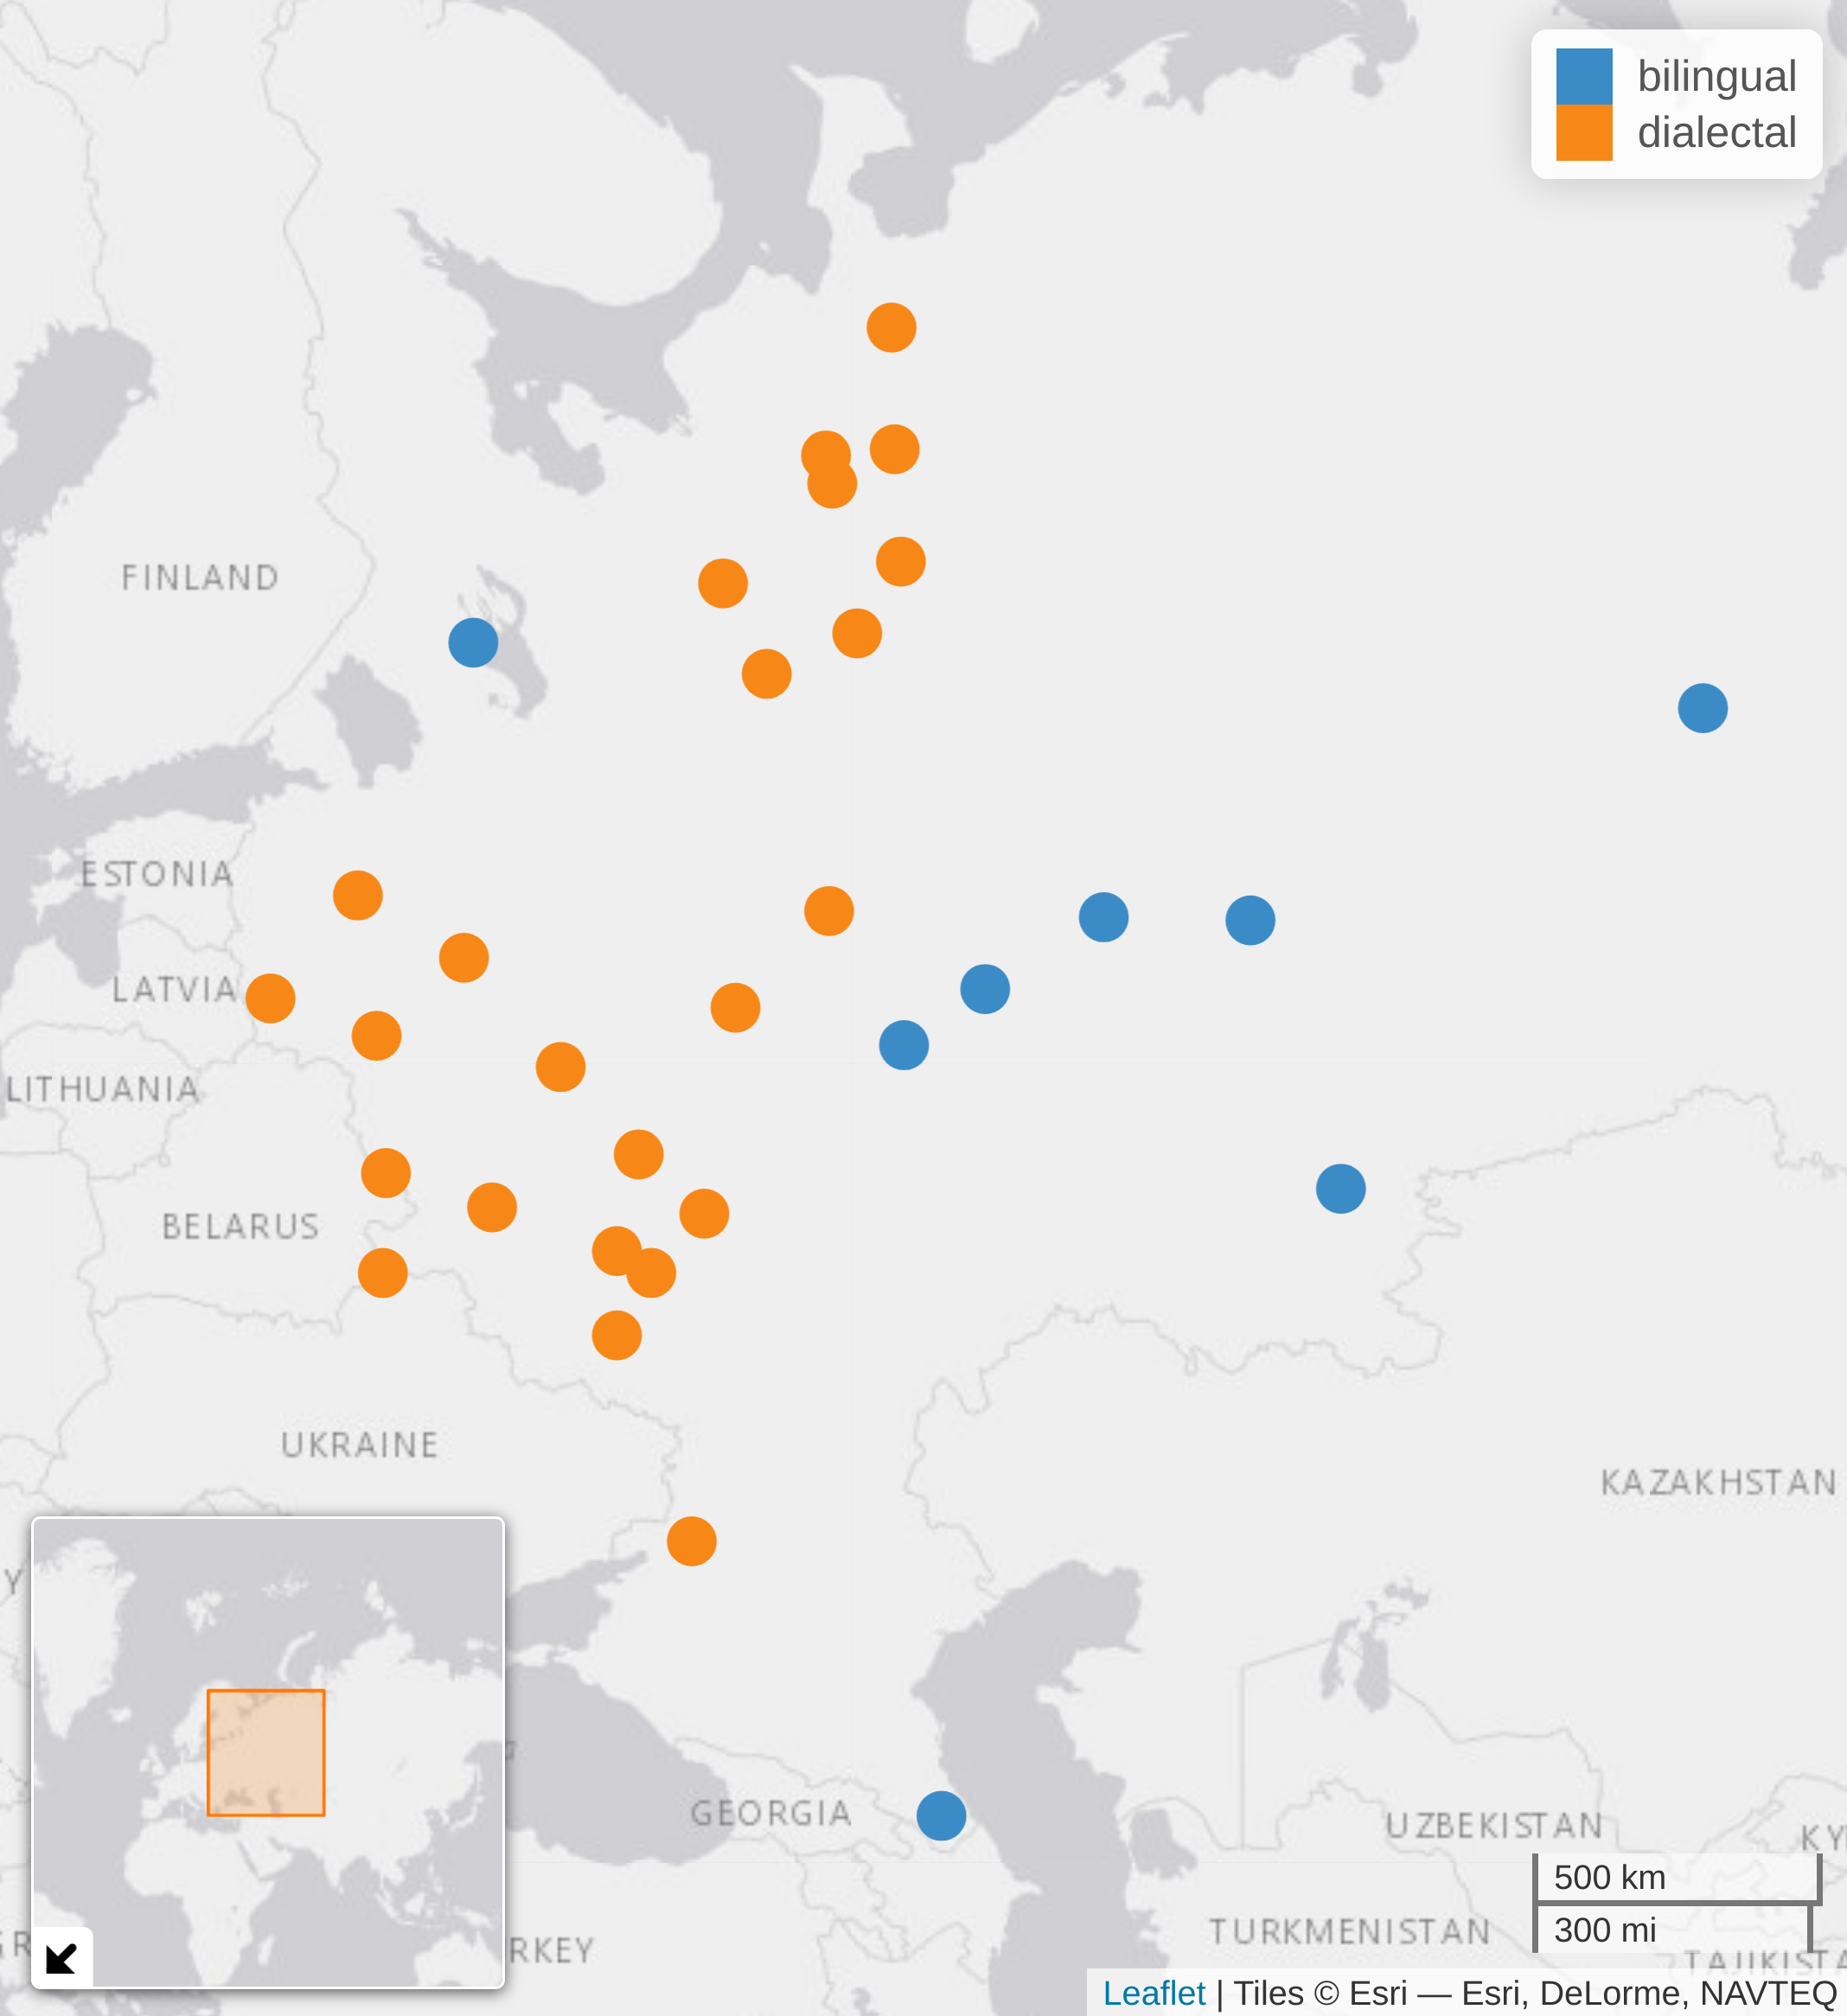
\includegraphics[width=7.12in,height=0.85\textheight]{images/map.png}

}

\caption{Created with \texttt{lingtypology} \citep{moroz17}}

\end{figure}%
\end{frame}

\begin{frame}{}
\phantomsection\label{section}
\vfill
\centering \LARGE

\alert{Can we analyze variation of linguistic features across all corpora?}
\pause

\alert{What are the factors that influence variation?} \pause

\alert{Can we find different variation patterns?} \vfill
\end{frame}

\begin{frame}{Previous publications}
\phantomsection\label{previous-publications}
\begin{itemize}
\tightlist
\item
  Daghestanian Russian \citep{daniel10, panova21}
\item
  Russian of Erzya speakers \citep{shagal16}
\item
  Russian of Kazakh speakers \citep{rakhilina18}
\item
  Contact Russian of Northern Siberia and the Russian Far East
  \citep{stoynova19, stoynova21}
\item
  Russian of Moksha speakers \citep{kashkin20}
\item
  Russian of Hill Mari \citep{kashkin22}
\item
  Russian of Nganasan speakers \citep{khomchenkova20}
\end{itemize}
\end{frame}

\section{The DiaL2 project}\label{the-dial2-project}

\begin{frame}{The DiaL2 team}
\phantomsection\label{the-dial2-team}
\begin{figure}

\begin{minipage}{0.25\linewidth}

\begin{figure}[H]

{\centering 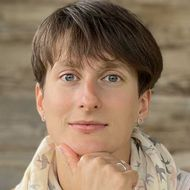
\includegraphics[width=0.63in,height=\textheight]{images/yermolova.jpeg}

}

\subcaption{Maria Ermolova}

\end{figure}%

\end{minipage}%
%
\begin{minipage}{0.25\linewidth}

\begin{figure}[H]

{\centering 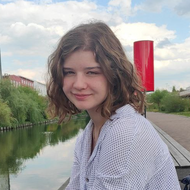
\includegraphics[width=0.63in,height=\textheight]{images/grishanova.png}

}

\subcaption{Anna Grishanova}

\end{figure}%

\end{minipage}%
%
\begin{minipage}{0.25\linewidth}

\begin{figure}[H]

{\centering 
\includegraphics[width=0.63in,height=\textheight]{images/koshelyuk.jpeg}

}

\subcaption{Natalia Koshelyuk}

\end{figure}%

\end{minipage}%
%
\begin{minipage}{0.25\linewidth}

\begin{figure}[H]

{\centering 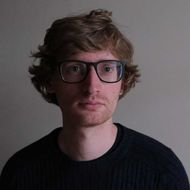
\includegraphics[width=0.63in,height=\textheight]{images/moroz.jpeg}

}

\subcaption{George Moroz}

\end{figure}%

\end{minipage}%
\newline
\begin{minipage}{0.25\linewidth}

\begin{figure}[H]

{\centering 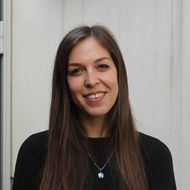
\includegraphics[width=0.63in,height=\textheight]{images/naccarato.jpg}

}

\subcaption{Chiara Naccarato}

\end{figure}%

\end{minipage}%
%
\begin{minipage}{0.25\linewidth}

\begin{figure}[H]

{\centering 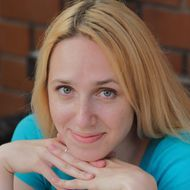
\includegraphics[width=0.63in,height=\textheight]{images/yakovleva.jpg}

}

\subcaption{Anastasia Yakovleva}

\end{figure}%

\end{minipage}%
%
\begin{minipage}{0.25\linewidth}

\begin{figure}[H]

{\centering 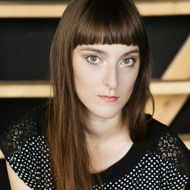
\includegraphics[width=0.63in,height=\textheight]{images/zemicheva.jpeg}

}

\subcaption{Svetlana Zemicheva}

\end{figure}%

\end{minipage}%

\end{figure}%
\end{frame}

\begin{frame}{The DiaL2 pipeline}
\phantomsection\label{the-dial2-pipeline}
\end{frame}

\section{The DiaL2 results}\label{the-dial2-results}

\begin{frame}{Some results}
\phantomsection\label{some-results}
\begin{itemize}
\tightlist
\item
  Non-standard numeral constructions in L2 Russian
\item
  Propositional Drop
\item
  Propositional Drop in Chuvash
\item
  Dialect Genitive Plural Forms of Masculine and Neuter Nouns in Numeral
  Constructions
\item
  Negative Existential Constructions
\end{itemize}
\end{frame}

\begin{frame}{Non-standard numeral constructions in L2 Russian}
\phantomsection\label{non-standard-numeral-constructions-in-l2-russian}
\begin{figure}

\begin{minipage}{0.50\linewidth}

\begin{figure}[H]

{\centering 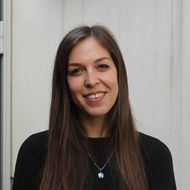
\includegraphics[width=0.63in,height=\textheight]{images/naccarato.jpg}

}

\subcaption{Chiara Naccarato}

\end{figure}%

\end{minipage}%
%
\begin{minipage}{0.50\linewidth}

\begin{figure}[H]

{\centering 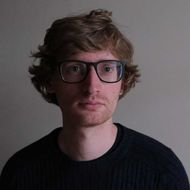
\includegraphics[width=0.63in,height=\textheight]{images/moroz.jpeg}

}

\subcaption{George Moroz}

\end{figure}%

\end{minipage}%

\end{figure}%
\end{frame}

\begin{frame}{Non-standard numeral constructions in L2 Russian}
\phantomsection\label{non-standard-numeral-constructions-in-l2-russian-1}
\begin{itemize}
\tightlist
\item
  Variation in numeral constructions (NCs) in bilingual corpora

  \begin{itemize}
  \tightlist
  \item
    e.g.~dva brat vs.~dva brata
  \end{itemize}
\item
  Previous research on other L2 Russian varieties

  \begin{itemize}
  \tightlist
  \item
    Stoynova (2021) on Nanai and Ulcha Russian: evidence for pattern
    borrowing
  \end{itemize}
\item
  Also mentioned by

  \begin{itemize}
  \tightlist
  \item
    Shagal (2016: 369-370) for Erzya Russian
  \item
    Rakhilina \& Kazkenova (2018: 610) for Kazakh Russian
  \end{itemize}
\end{itemize}
\end{frame}

\begin{frame}{Research questions}
\phantomsection\label{research-questions}
\begin{itemize}
\tightlist
\item
  Does the amount of variation in NCs differ across corpora and/or among
  speakers of the same variety?
\item
  Can variation in NCs be explained in terms of contact influence?
\item
  Do other factors promote or hinder variation in NCs?
\end{itemize}
\end{frame}

\begin{frame}{The database and parameters of data annotation}
\phantomsection\label{the-database-and-parameters-of-data-annotation}
4,144 observations

\begin{center}
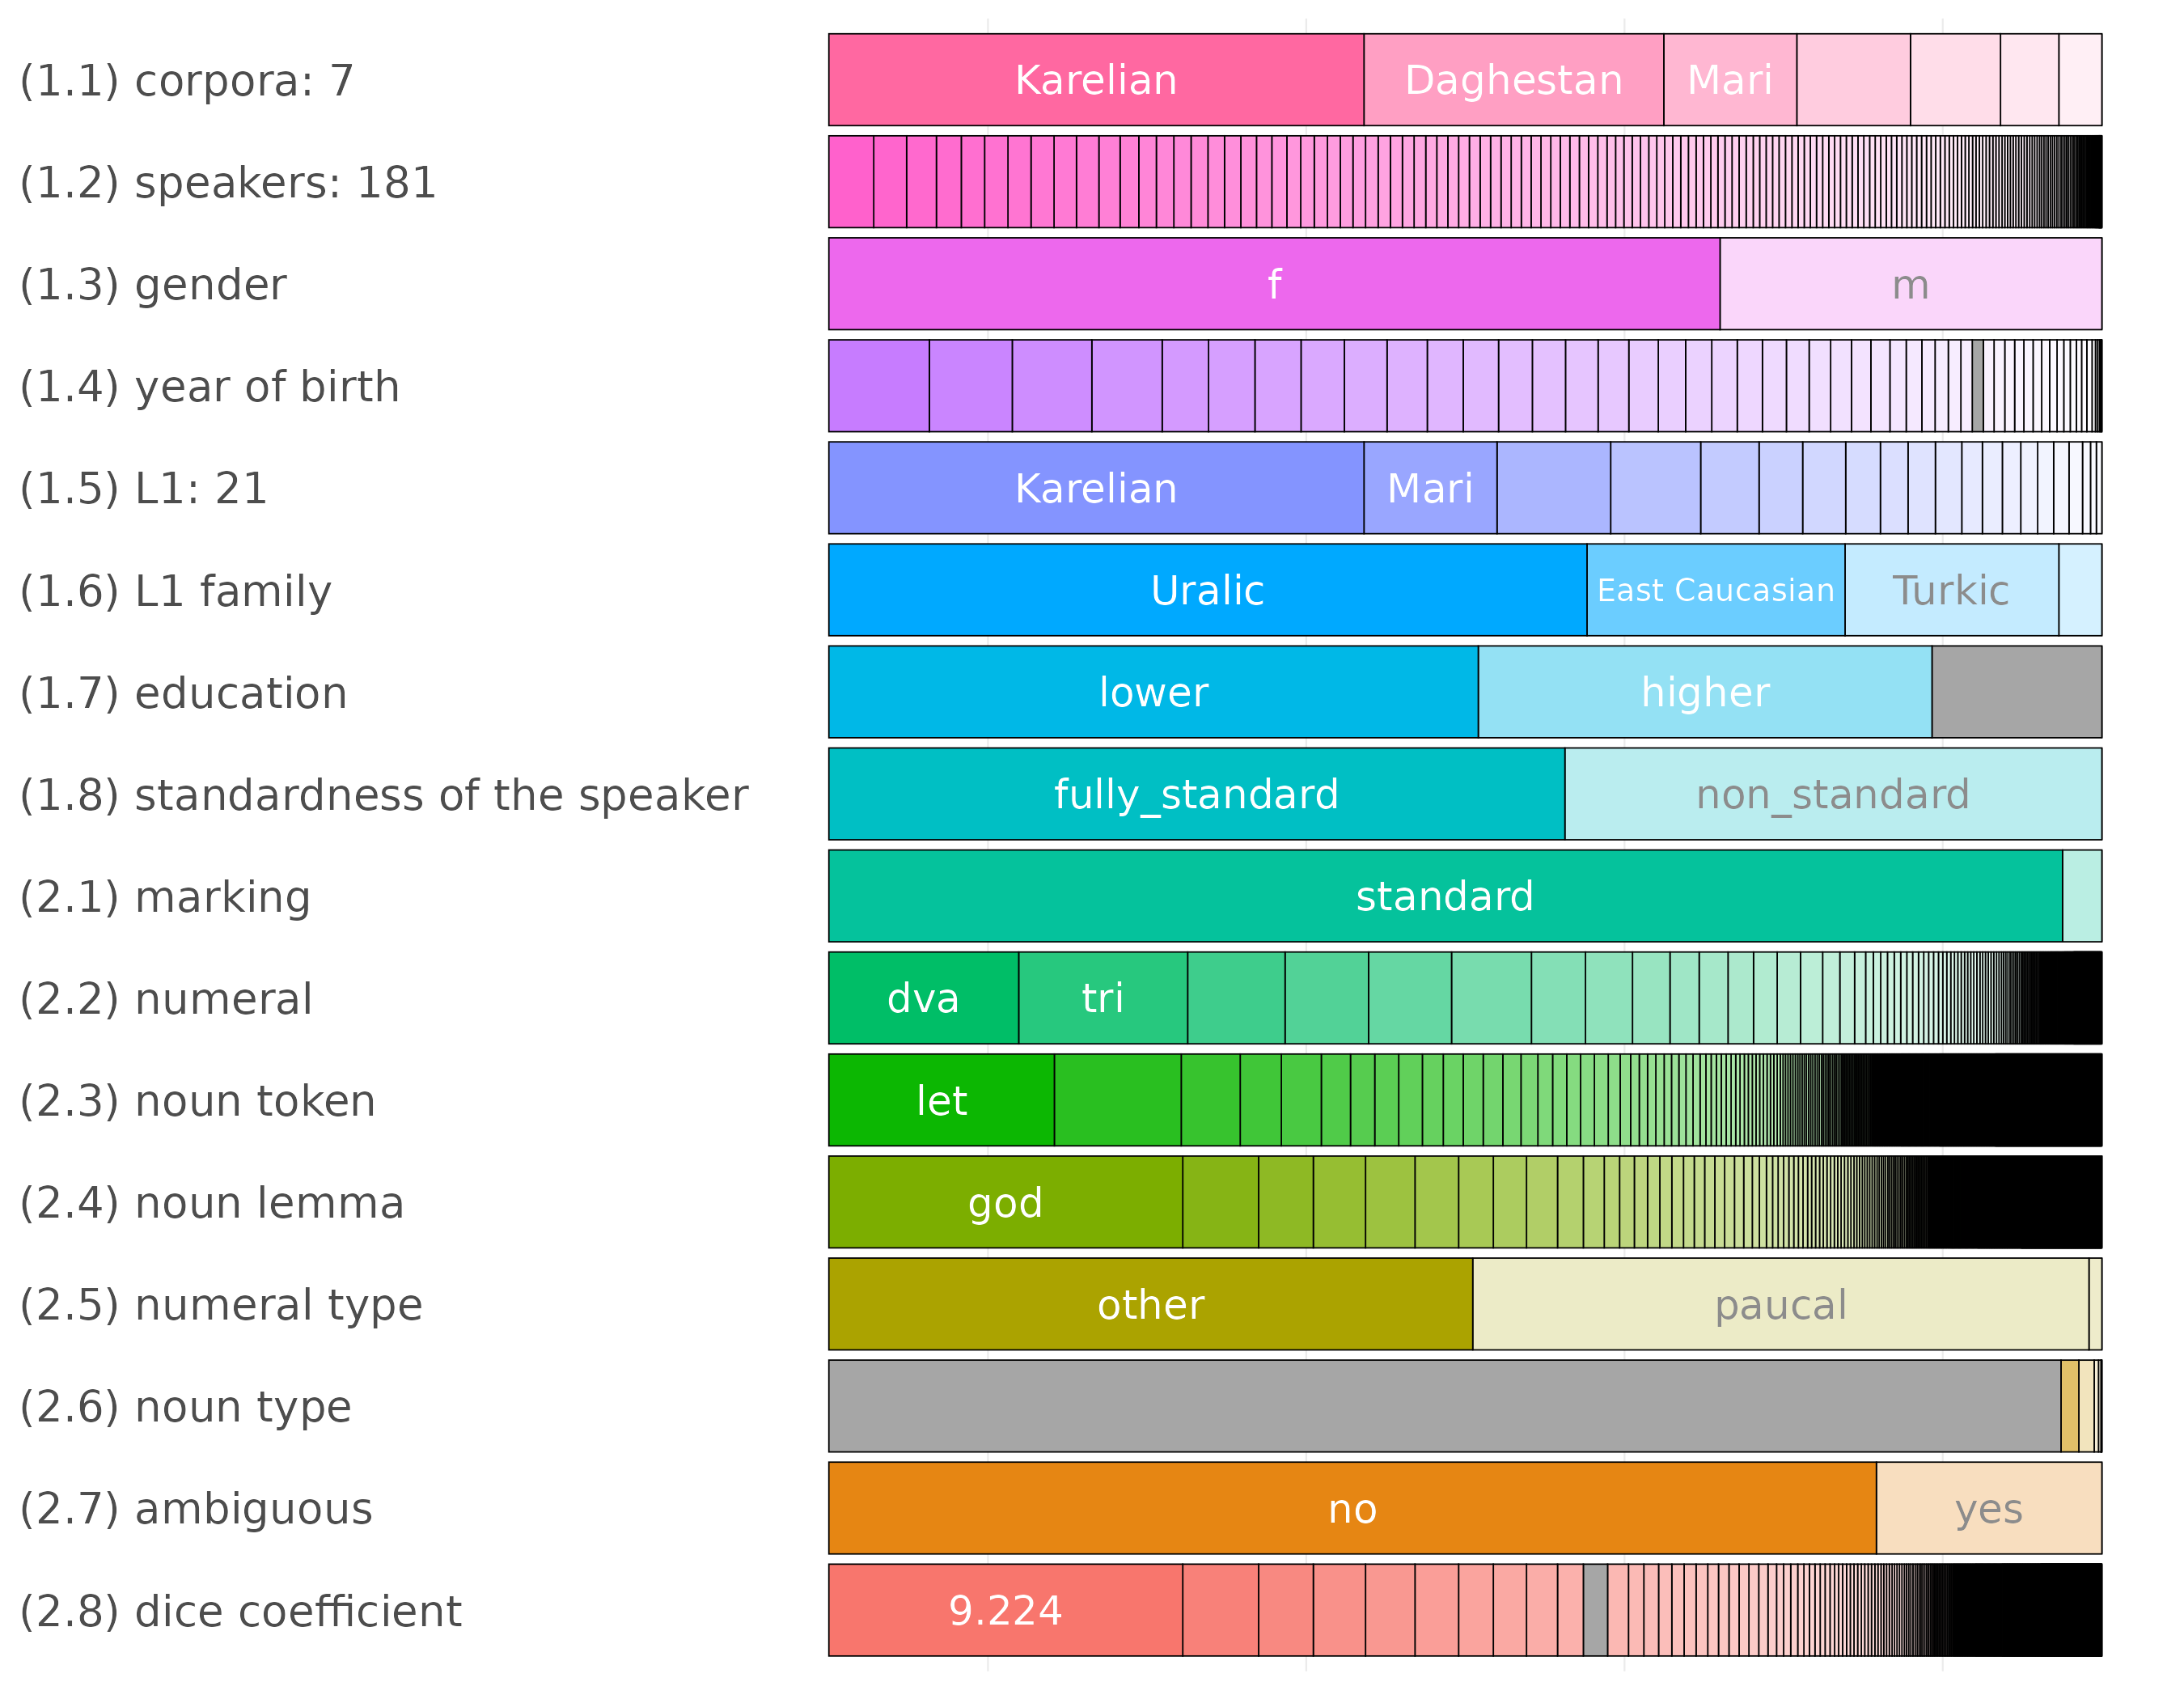
\includegraphics[width=9in,height=0.84\textheight]{images/l2_num_constr_df_structure.png}
\end{center}
\end{frame}

\begin{frame}{Fully standard (71.3\%) vs.~non-standard speakers
(28.7\%)}
\phantomsection\label{fully-standard-71.3-vs.-non-standard-speakers-28.7}
\begin{center}
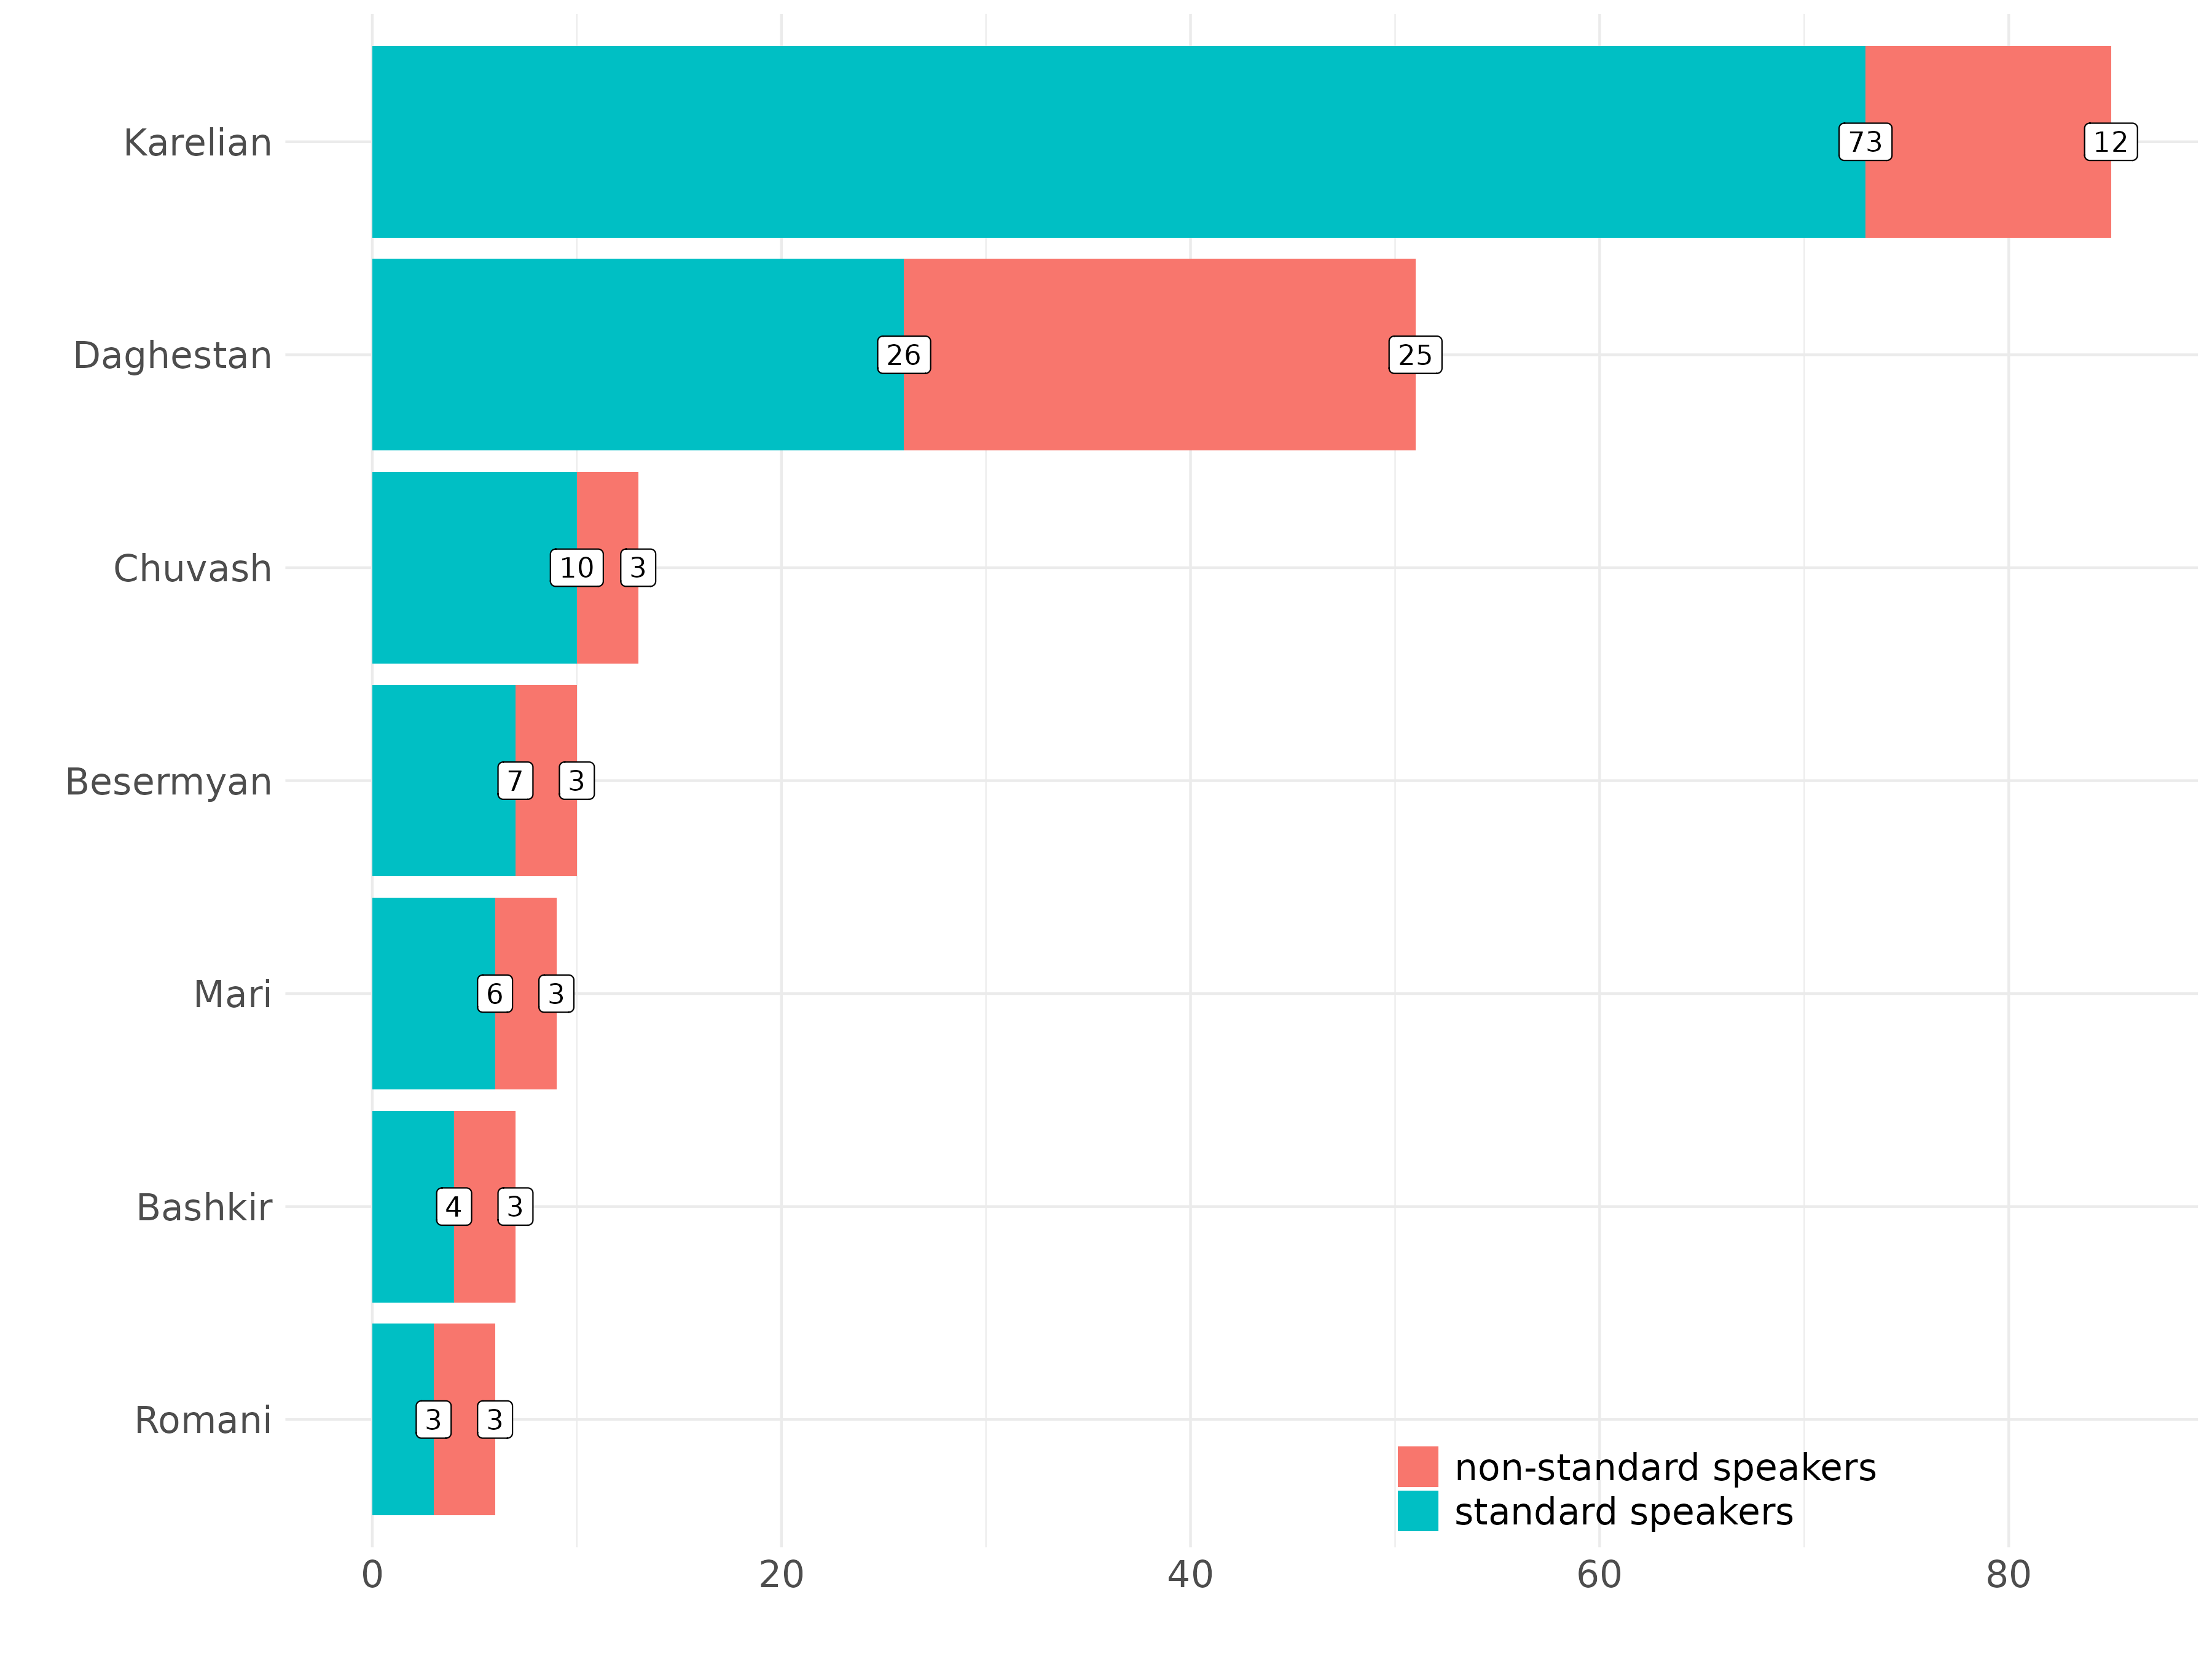
\includegraphics[width=12in,height=0.93\textheight]{images/l2_num_constr_distribution_of_speakers_by_standardness_across_corpora.png}
\end{center}
\end{frame}

\begin{frame}{Proportion of non-standard occurrences per corpus}
\phantomsection\label{proportion-of-non-standard-occurrences-per-corpus}
1,748 observations

\begin{center}
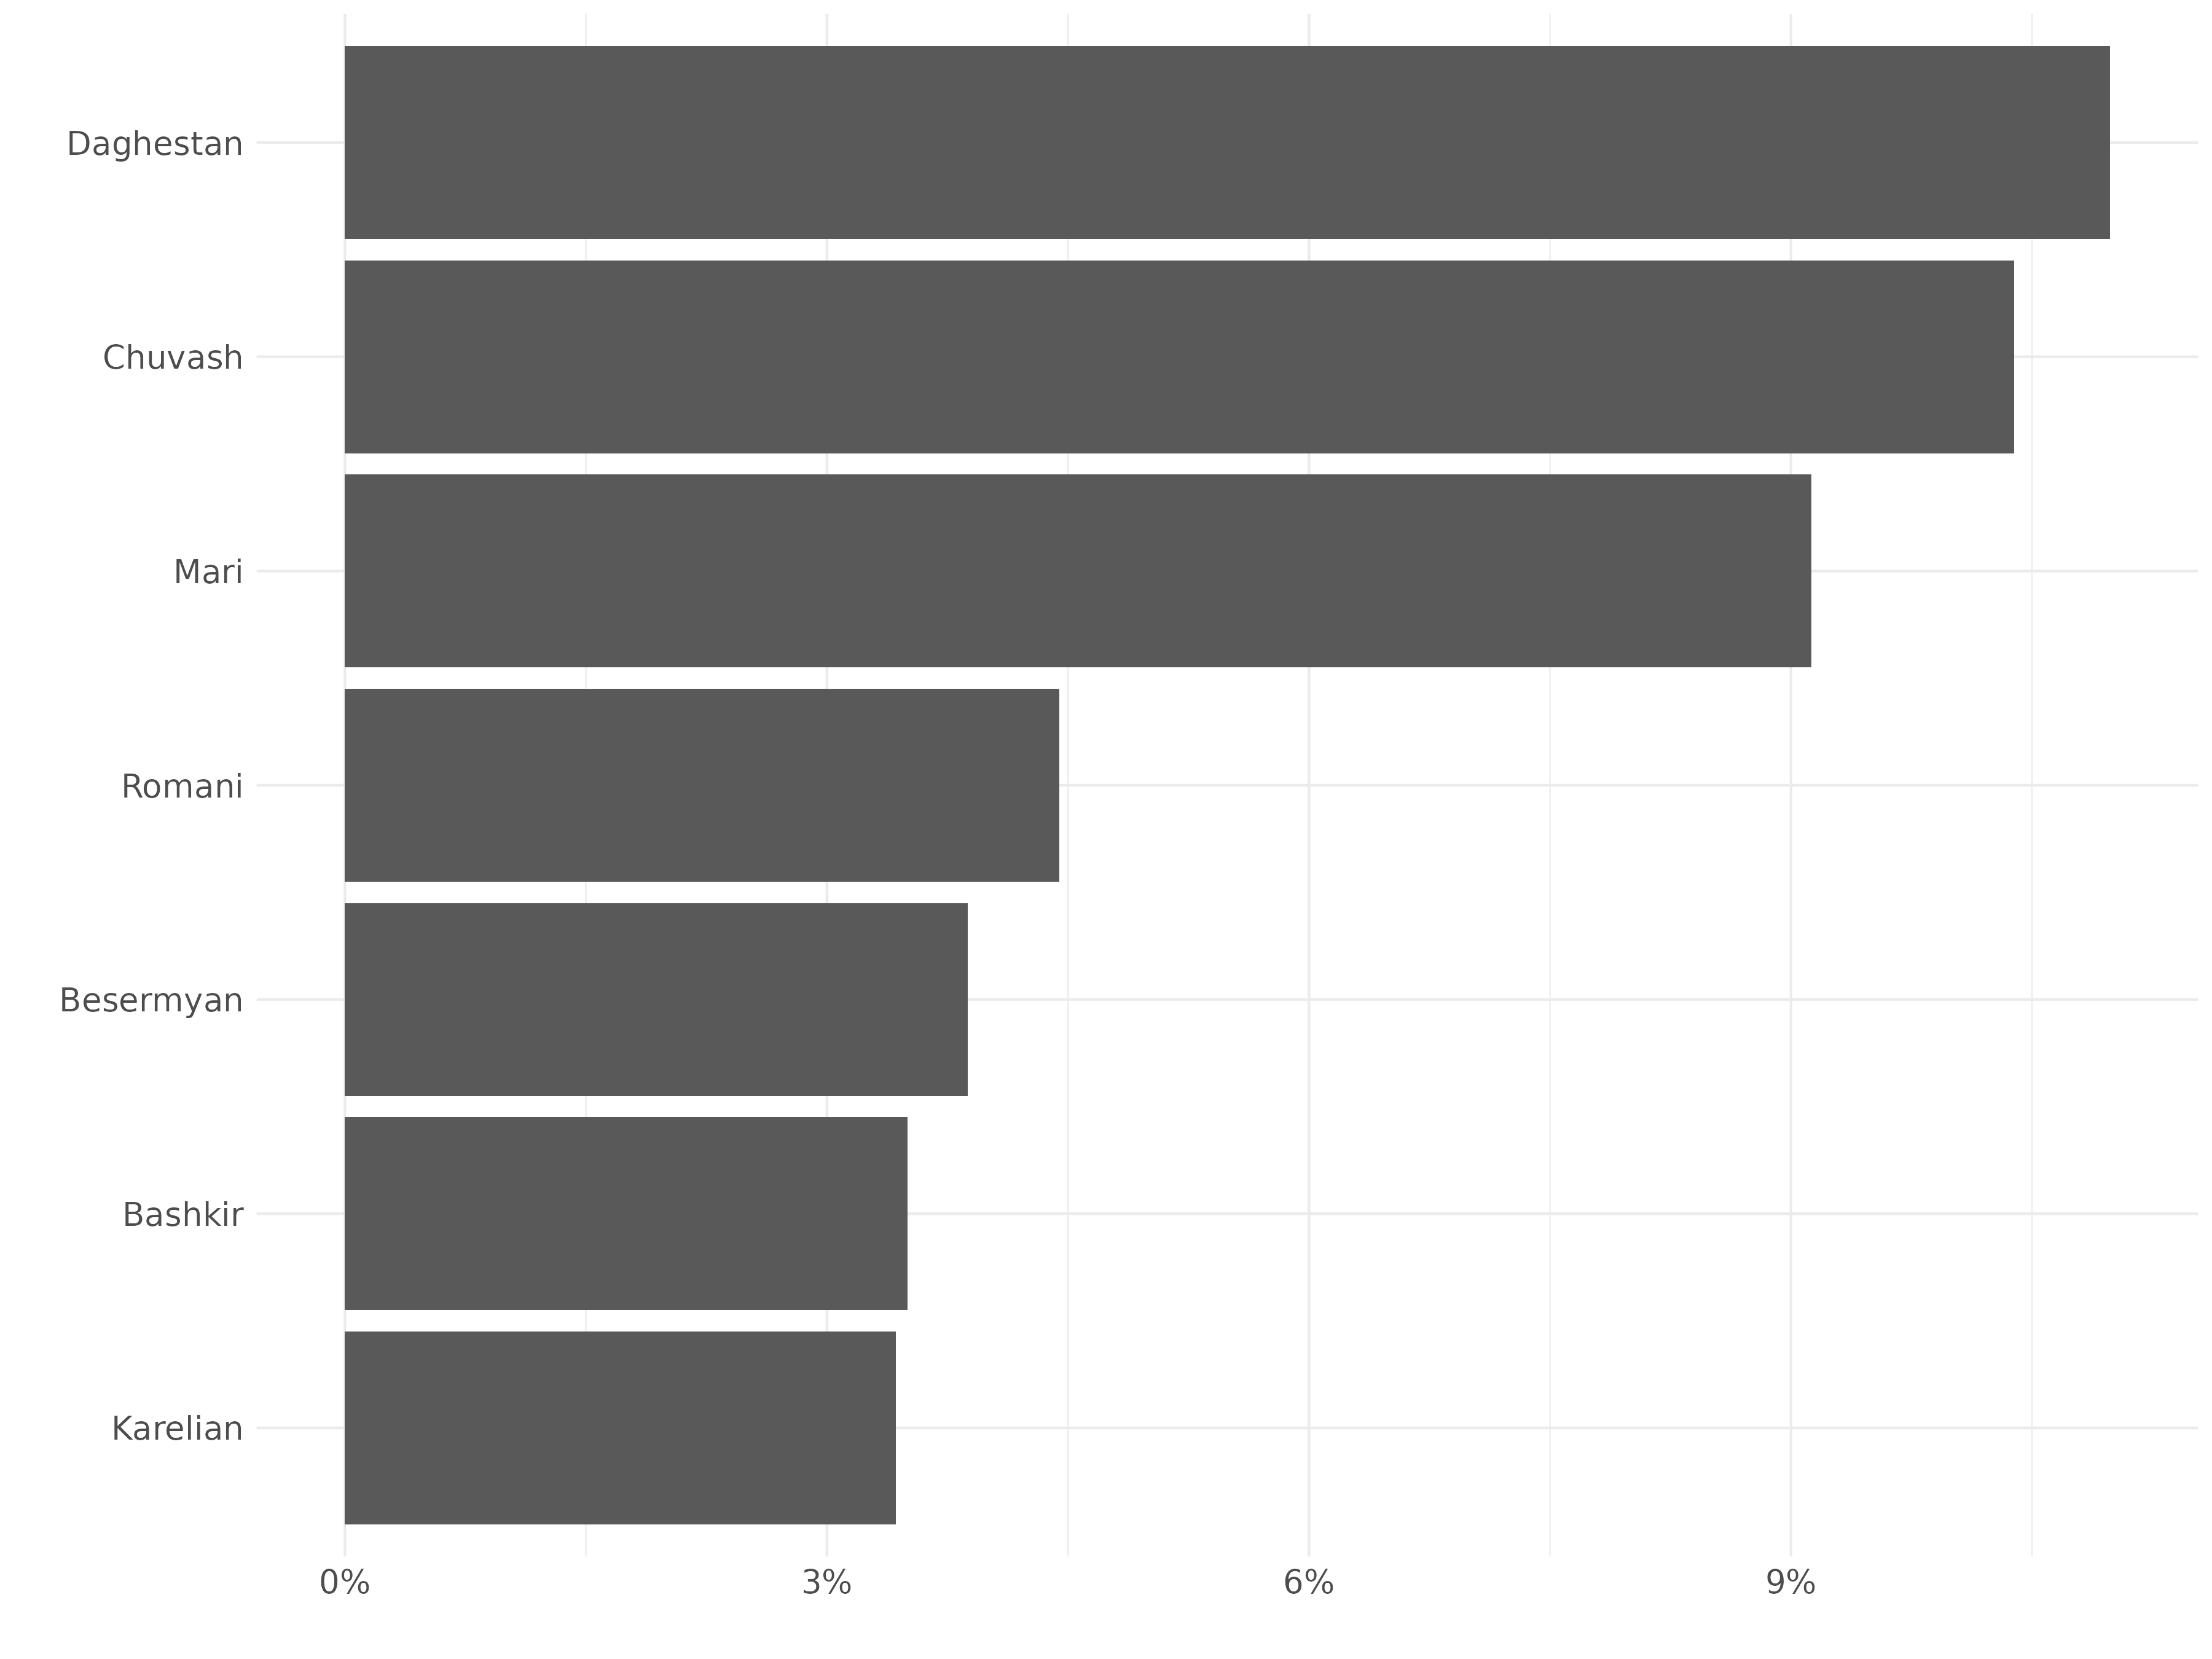
\includegraphics[width=12in,height=0.84\textheight]{images/l2_num_constr_distribution_of_nstd_forms_without_fully_std_speakers.png}
\end{center}
\end{frame}

\begin{frame}{Distribution of n-std forms with different types of
numerals}
\phantomsection\label{distribution-of-n-std-forms-with-different-types-of-numerals}
\begin{figure}

\begin{minipage}{0.35\linewidth}

\begin{itemize}
\tightlist
\item
  NOM instead of GEN is frequent both with paucals and other numerals
\item
  n-std GEN is attested sporadically
\item
  other case forms are even less frequent
\item
  only \textasciitilde45\% of n-std expressions could in principle be
  explained by L1 pattern borrowing
\end{itemize}

\end{minipage}%
%
\begin{minipage}{0.65\linewidth}

\begin{center}
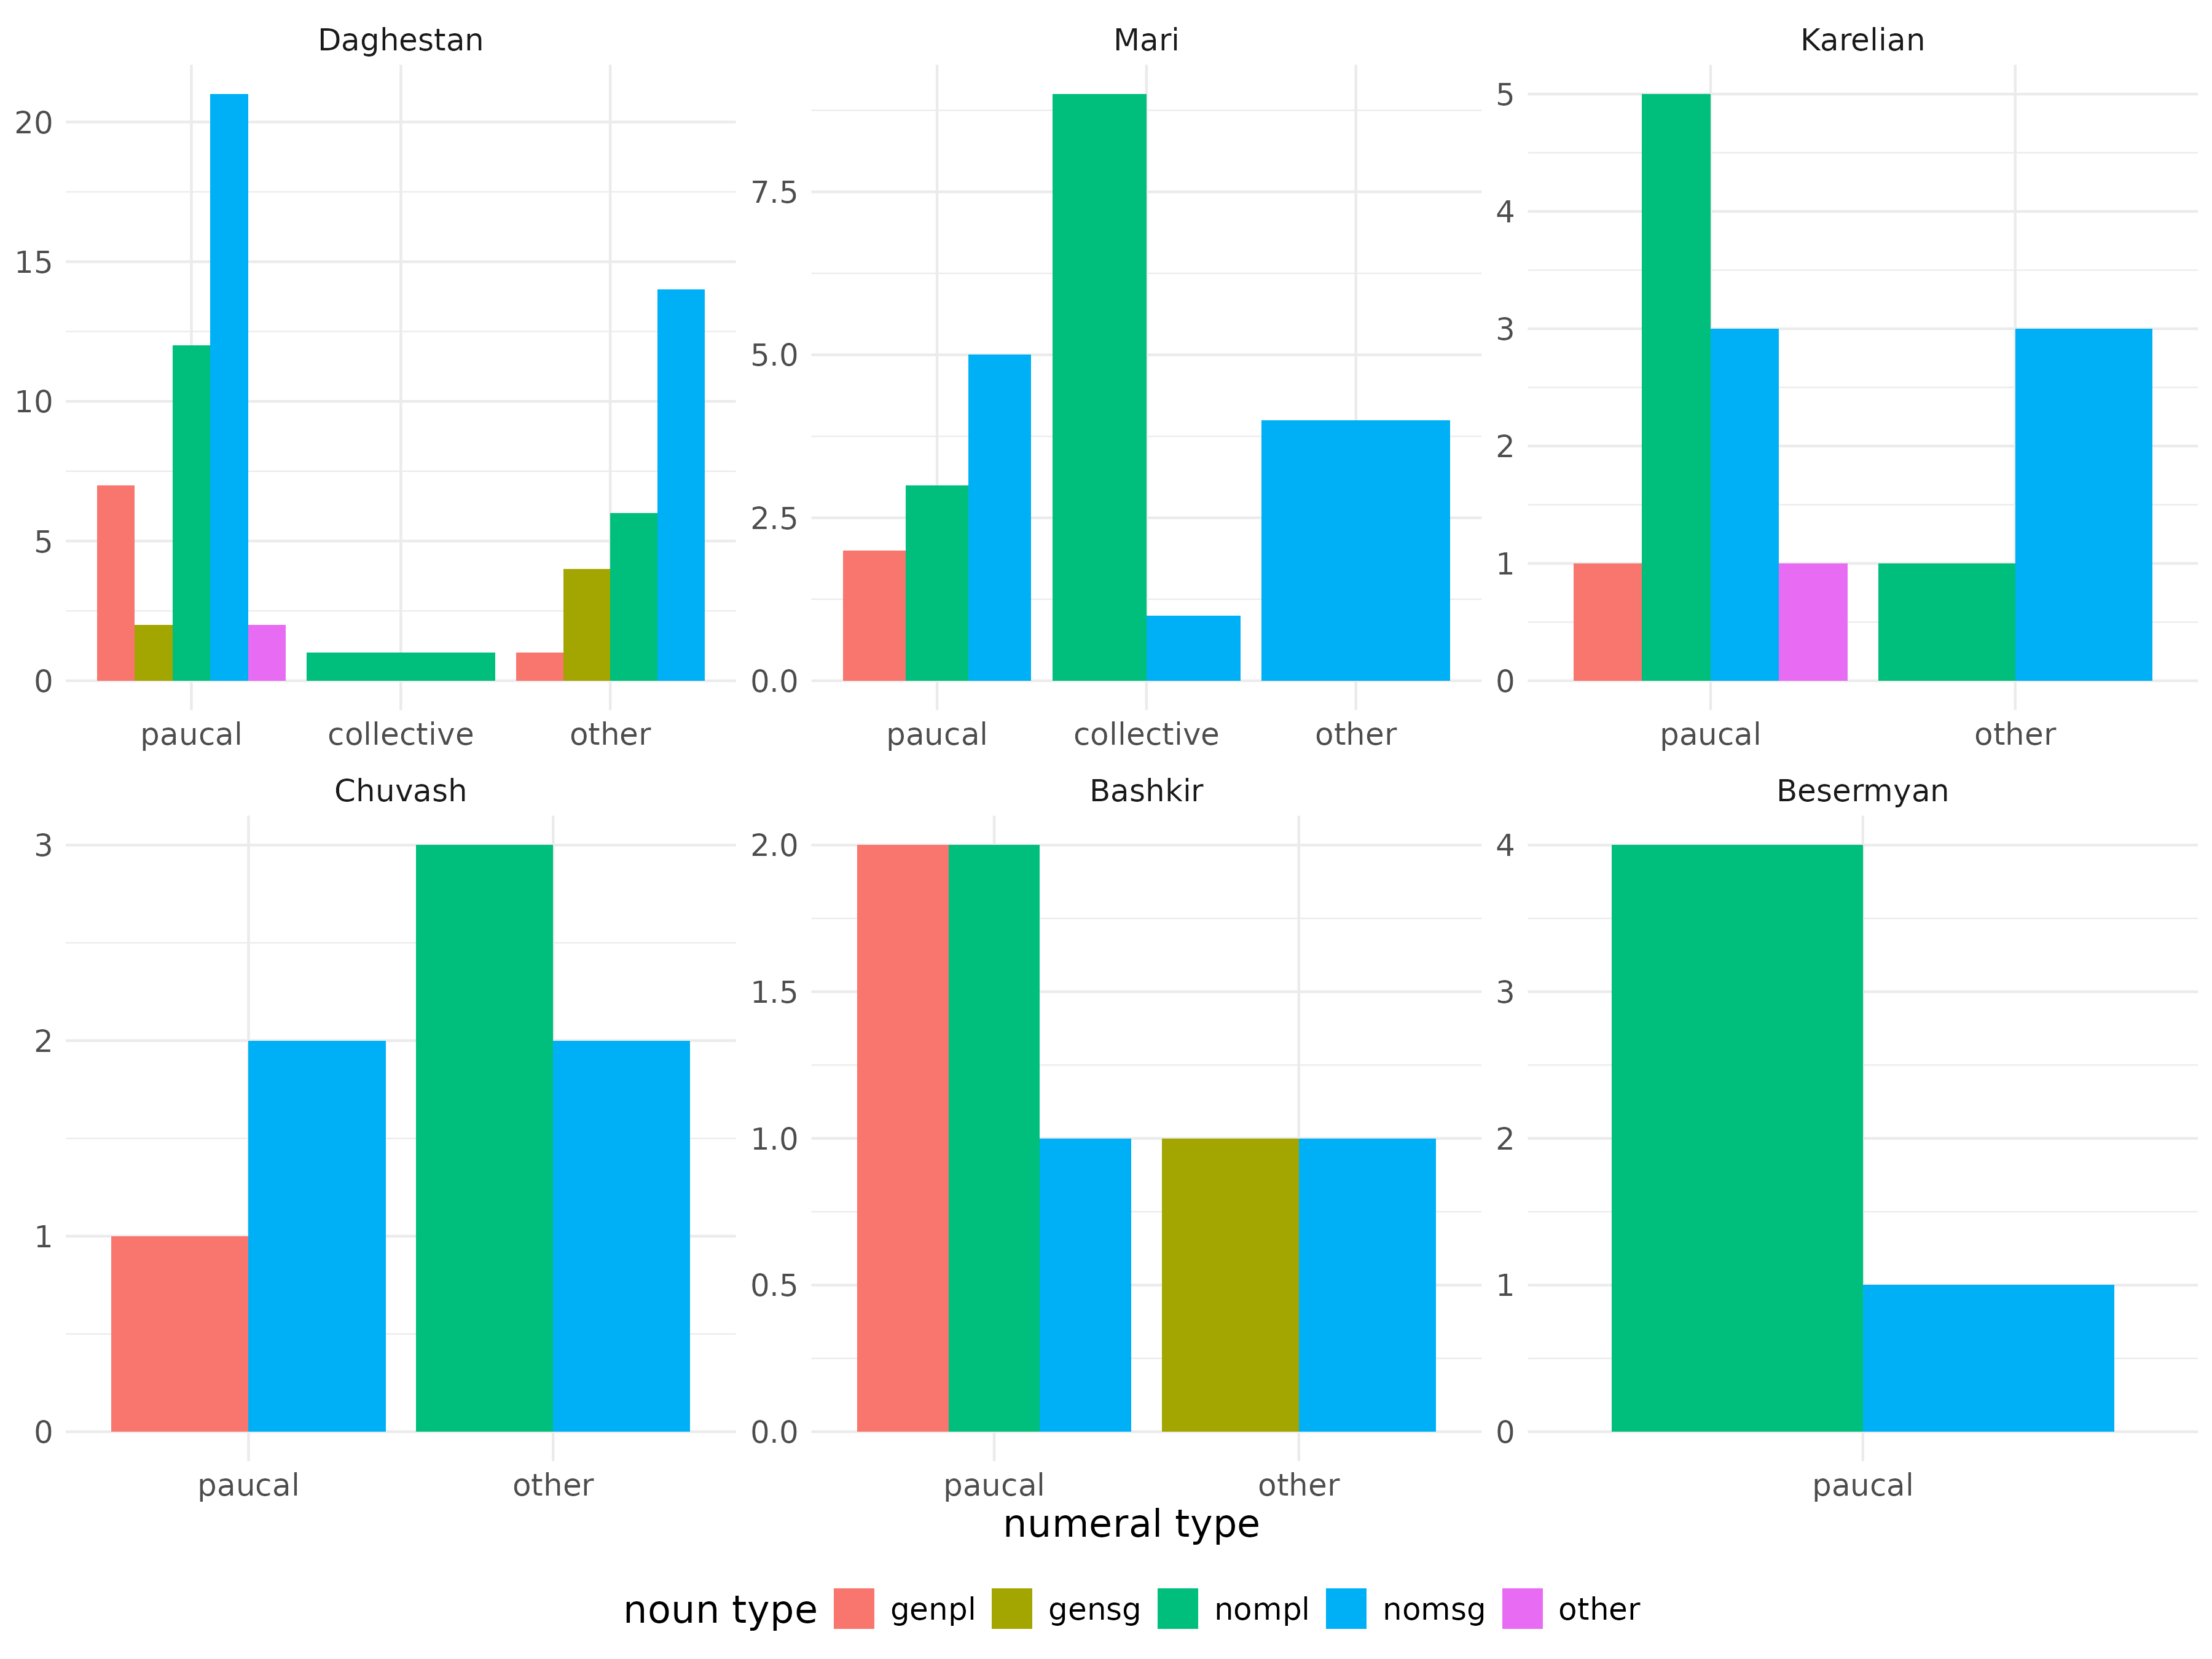
\includegraphics[width=1.1\textwidth,height=\textheight]{images/l2_num_constr_distribution_of_nstd_forms_with_different_types_of_numerals.png}
\end{center}

\end{minipage}%

\end{figure}%
\end{frame}

\begin{frame}[fragile]{Statistical modelling}
\phantomsection\label{statistical-modelling}
\begin{center}
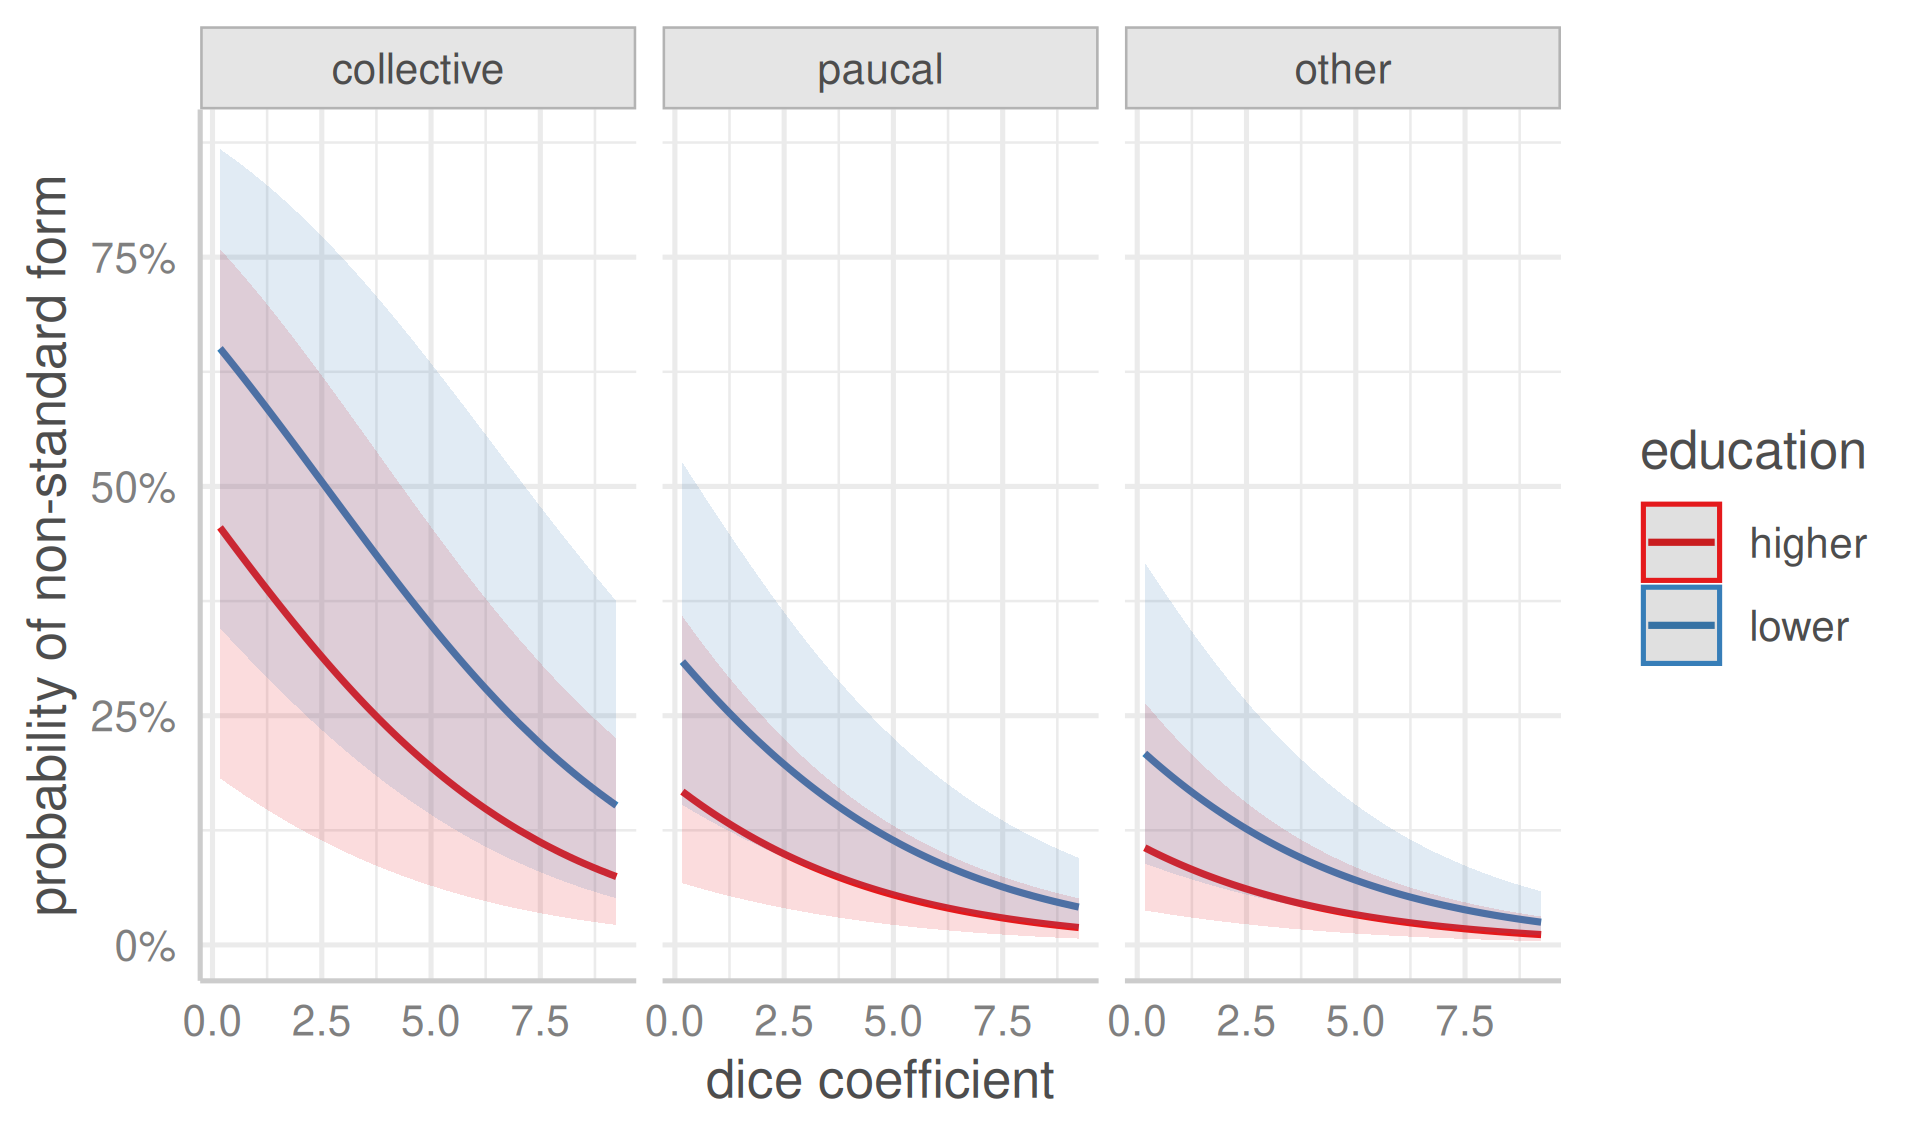
\includegraphics[width=0.8\textwidth,height=\textheight]{images/l2_num_constr_model_prediction_by_dice_coefficient_education_num_type.png}
\end{center}

\begin{itemize}
\tightlist
\item
  Logistic regression:
  \small \texttt{standardness\ \textasciitilde{}\ Dice\ coefficient\ +\ year\ of\ birth\ +\ education\ +\ numeral\ type\ +\ gender\ +\ (1\textbar{}L1\ family/speaker\ id)}
  \normalsize
\item
  Conditional importance of the variables in our model (generalized R
  squared): collocationality (Dice coefficient) \textgreater{} education
  \textgreater{} year of birth \textgreater{} numeral type
  \textgreater{} gender
\end{itemize}
\end{frame}

\begin{frame}{Conclusions}
\phantomsection\label{conclusions}
\begin{itemize}
\tightlist
\item
  Variation in NCs is attested in all L2 corpora, but not to the same
  extent in each of them
\item
  Daghestanian Russian as a more uniform variety, probably due to a
  lower pervasiveness of Russian in every-day life, especially in the
  more isolated communities of the highlands
\item
  The variables that turned out to be statistically significant are all
  logically related to L2 proficiency and exposure to the input, but
  there is no robust evidence for a contact explanation
\end{itemize}
\end{frame}

\begin{frame}{Propositional Drop}
\phantomsection\label{propositional-drop}
\begin{figure}

\begin{minipage}{0.33\linewidth}

\begin{figure}[H]

{\centering 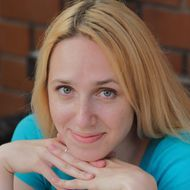
\includegraphics[width=0.63in,height=\textheight]{images/yakovleva.jpg}

}

\subcaption{Anastasia Yakovleva}

\end{figure}%

\end{minipage}%
%
\begin{minipage}{0.33\linewidth}

\begin{figure}[H]

{\centering 
\includegraphics[width=0.63in,height=\textheight]{images/koshelyuk.jpeg}

}

\subcaption{Natalia Koshelyuk}

\end{figure}%

\end{minipage}%
%
\begin{minipage}{0.33\linewidth}

\begin{figure}[H]

{\centering 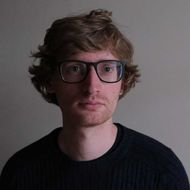
\includegraphics[width=0.63in,height=\textheight]{images/moroz.jpeg}

}

\subcaption{George Moroz}

\end{figure}%

\end{minipage}%

\end{figure}%
\end{frame}

\begin{frame}{Propositional Drop in Chuvash}
\phantomsection\label{propositional-drop-in-chuvash}
\begin{figure}[H]

{\centering 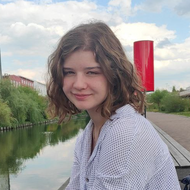
\includegraphics[width=0.63in,height=\textheight]{images/grishanova.png}

}

\caption{Anna Grishanova}

\end{figure}%
\end{frame}

\begin{frame}{Dialect Genitive Plural Forms in Numeral Constructions}
\phantomsection\label{dialect-genitive-plural-forms-in-numeral-constructions}
\begin{figure}

\begin{minipage}{0.33\linewidth}

\begin{figure}[H]

{\centering 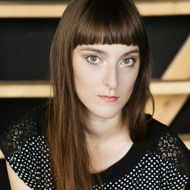
\includegraphics[width=0.63in,height=\textheight]{images/zemicheva.jpeg}

}

\subcaption{Svetlana Zemicheva}

\end{figure}%

\end{minipage}%
%
\begin{minipage}{0.33\linewidth}

\begin{figure}[H]

{\centering 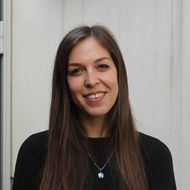
\includegraphics[width=0.63in,height=\textheight]{images/naccarato.jpg}

}

\subcaption{Chiara Naccarato}

\end{figure}%

\end{minipage}%
%
\begin{minipage}{0.33\linewidth}

\begin{figure}[H]

{\centering 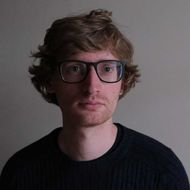
\includegraphics[width=0.63in,height=\textheight]{images/moroz.jpeg}

}

\subcaption{George Moroz}

\end{figure}%

\end{minipage}%

\end{figure}%
\end{frame}

\begin{frame}{Negative Existential Constructions}
\phantomsection\label{negative-existential-constructions}
\begin{figure}

\begin{minipage}{0.33\linewidth}

\begin{figure}[H]

{\centering 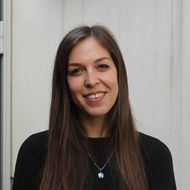
\includegraphics[width=0.63in,height=\textheight]{images/naccarato.jpg}

}

\subcaption{Chiara Naccarato}

\end{figure}%

\end{minipage}%
%
\begin{minipage}{0.33\linewidth}

\begin{figure}[H]

{\centering 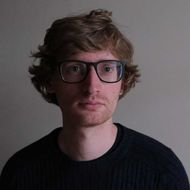
\includegraphics[width=0.63in,height=\textheight]{images/moroz.jpeg}

}

\subcaption{George Moroz}

\end{figure}%

\end{minipage}%

\end{figure}%
\end{frame}

\begin{frame}{Negative Existential Constructions}
\phantomsection\label{negative-existential-constructions-1}
\begin{itemize}
\tightlist
\item
  Existential negation = negation strategies used in existential
  sentences of the type \emph{there is/are no} X (\emph{somewhere}), in
  which the subject is typically non-referential
\item
  We use the terms ``existential negation'' and ``negative existential
  constructions'' (NECs) in a wider sense to include constructions that
  are sometimes referred to as ``locative negation'' (\emph{X is/are not
  in some place}, in which X is a definite subject) and ``possessive
  negation'' (\emph{Y does/do not have X}); cf.
  \citep[110--111]{veselinova13}
\item
  All of them predicate absolute absence rather than relative absence,
  and Russian employs one and the same strategy in all three cases,
  which is different from the strategy employed in standard negation,
  i.e.~negation of overt verb predicates
\end{itemize}
\end{frame}

\begin{frame}{Non-standard marking in NECs}
\phantomsection\label{non-standard-marking-in-necs}
\begin{itemize}
\tightlist
\item
  Variation in NECs in bilingual corpora (+ comparison with the
  monolinguals' variety of Russian spoken in Zvenigorod)
\end{itemize}

e.g.~\emph{gaz ne bylo} vs.~\emph{gaza ne bylo}

\begin{itemize}
\tightlist
\item
  Previous research on other L2 Russian varieties

  \begin{itemize}
  \tightlist
  \item
    Nanai and Ulcha Russian \citep[27]{stoynova19}
  \item
    Moksha Russian \citep[116]{kashkin20}
  \item
    Hill Mari Russian \citep[39]{kashkin22}
  \end{itemize}
\item
  Usually treated as a contact phenomenon because in the L1s of Russian
  bilinguals who display this trait there is no genitive (or any other
  special) marking of negated subjects
\end{itemize}
\end{frame}

\begin{frame}{Research questions}
\phantomsection\label{research-questions-1}
\begin{itemize}
\tightlist
\item
  Does the amount of variation in NECs differ across corpora and/or
  among speakers of the same variety?
\item
  Can variation in NECs be explained in terms of contact influence?
\item
  Do other factors promote or hinder variation in NECs?
\end{itemize}
\end{frame}

\begin{frame}{The database and parameters of data annotation}
\phantomsection\label{the-database-and-parameters-of-data-annotation-1}
2,309 observations

\begin{center}
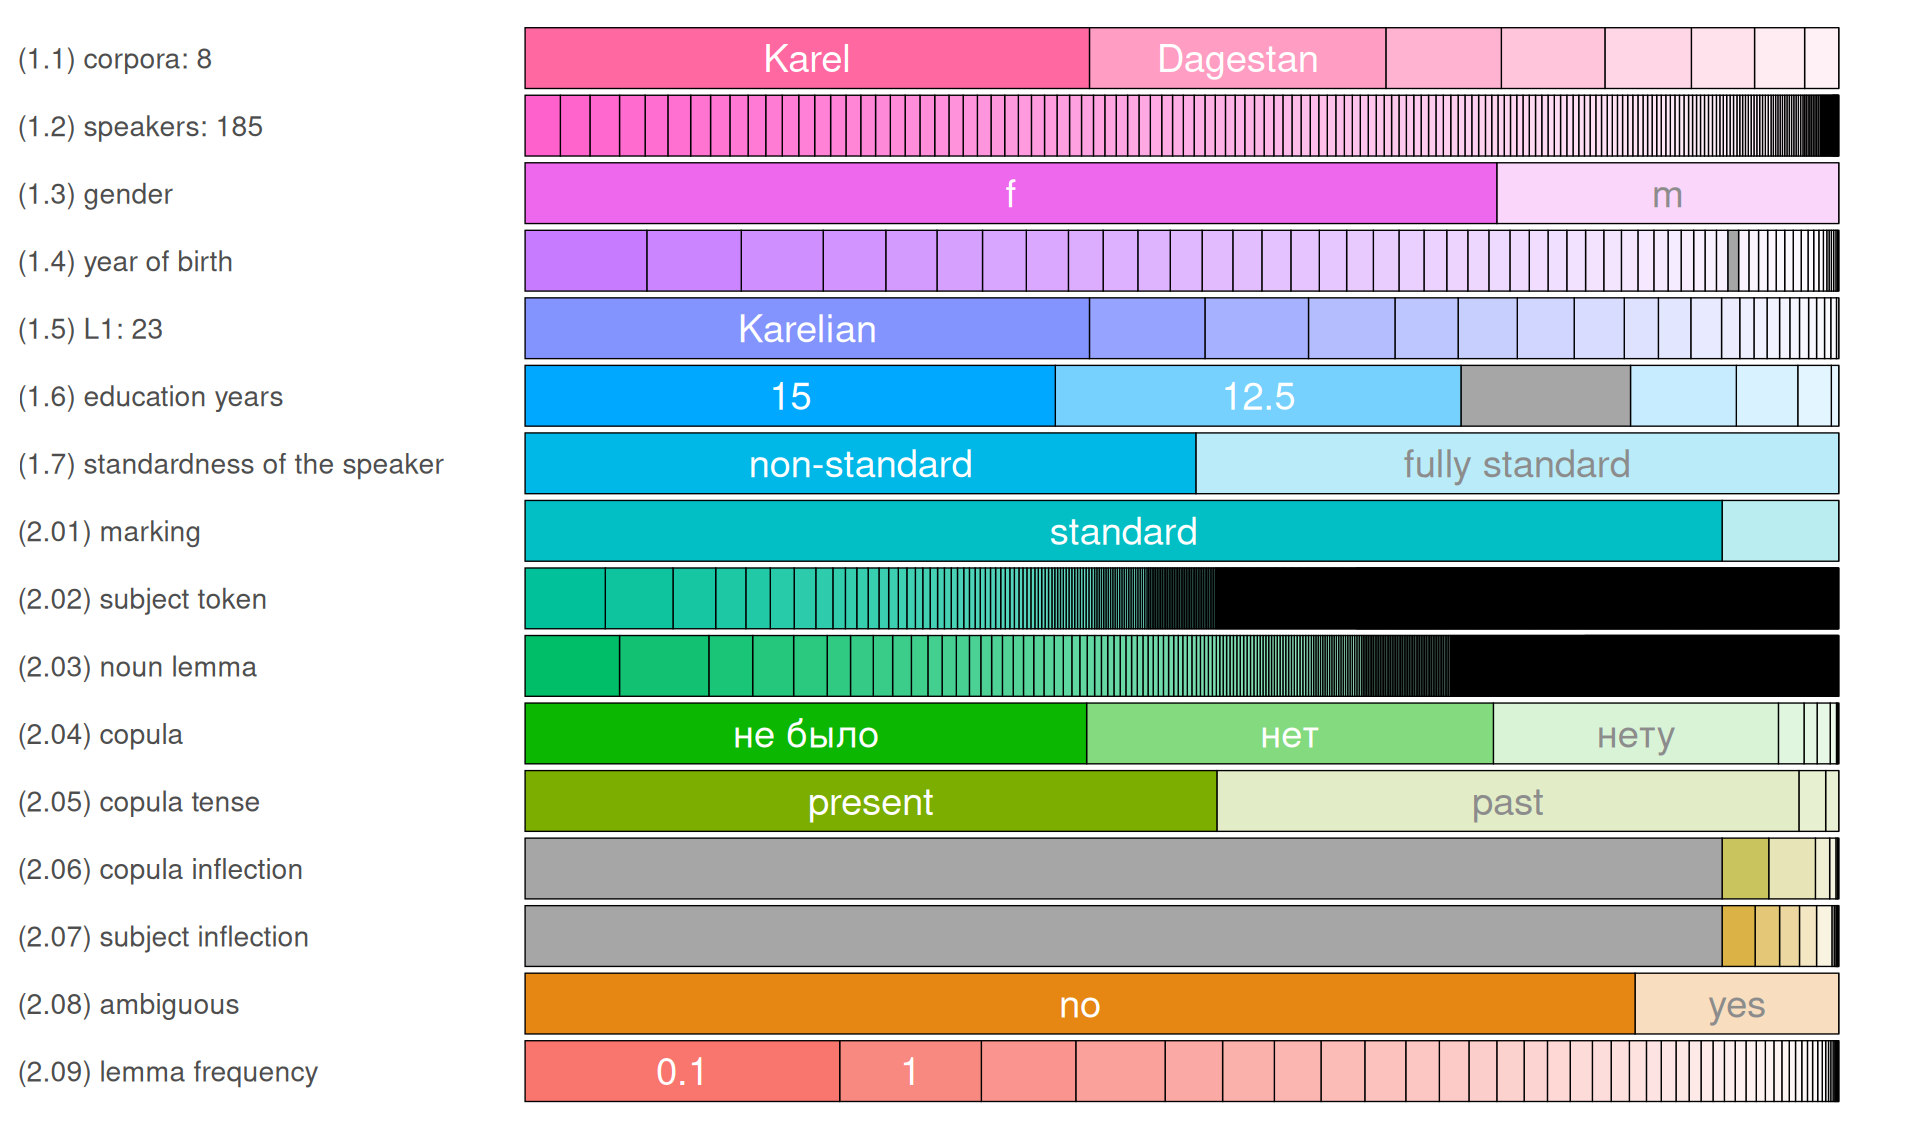
\includegraphics[width=1.05\textwidth,height=\textheight]{images/l2_neg_exist_constr_df_structure.png}
\end{center}
\end{frame}

\begin{frame}{Fully standard (58\%) vs.~non-standard speakers (42\%)}
\phantomsection\label{fully-standard-58-vs.-non-standard-speakers-42}
\begin{center}
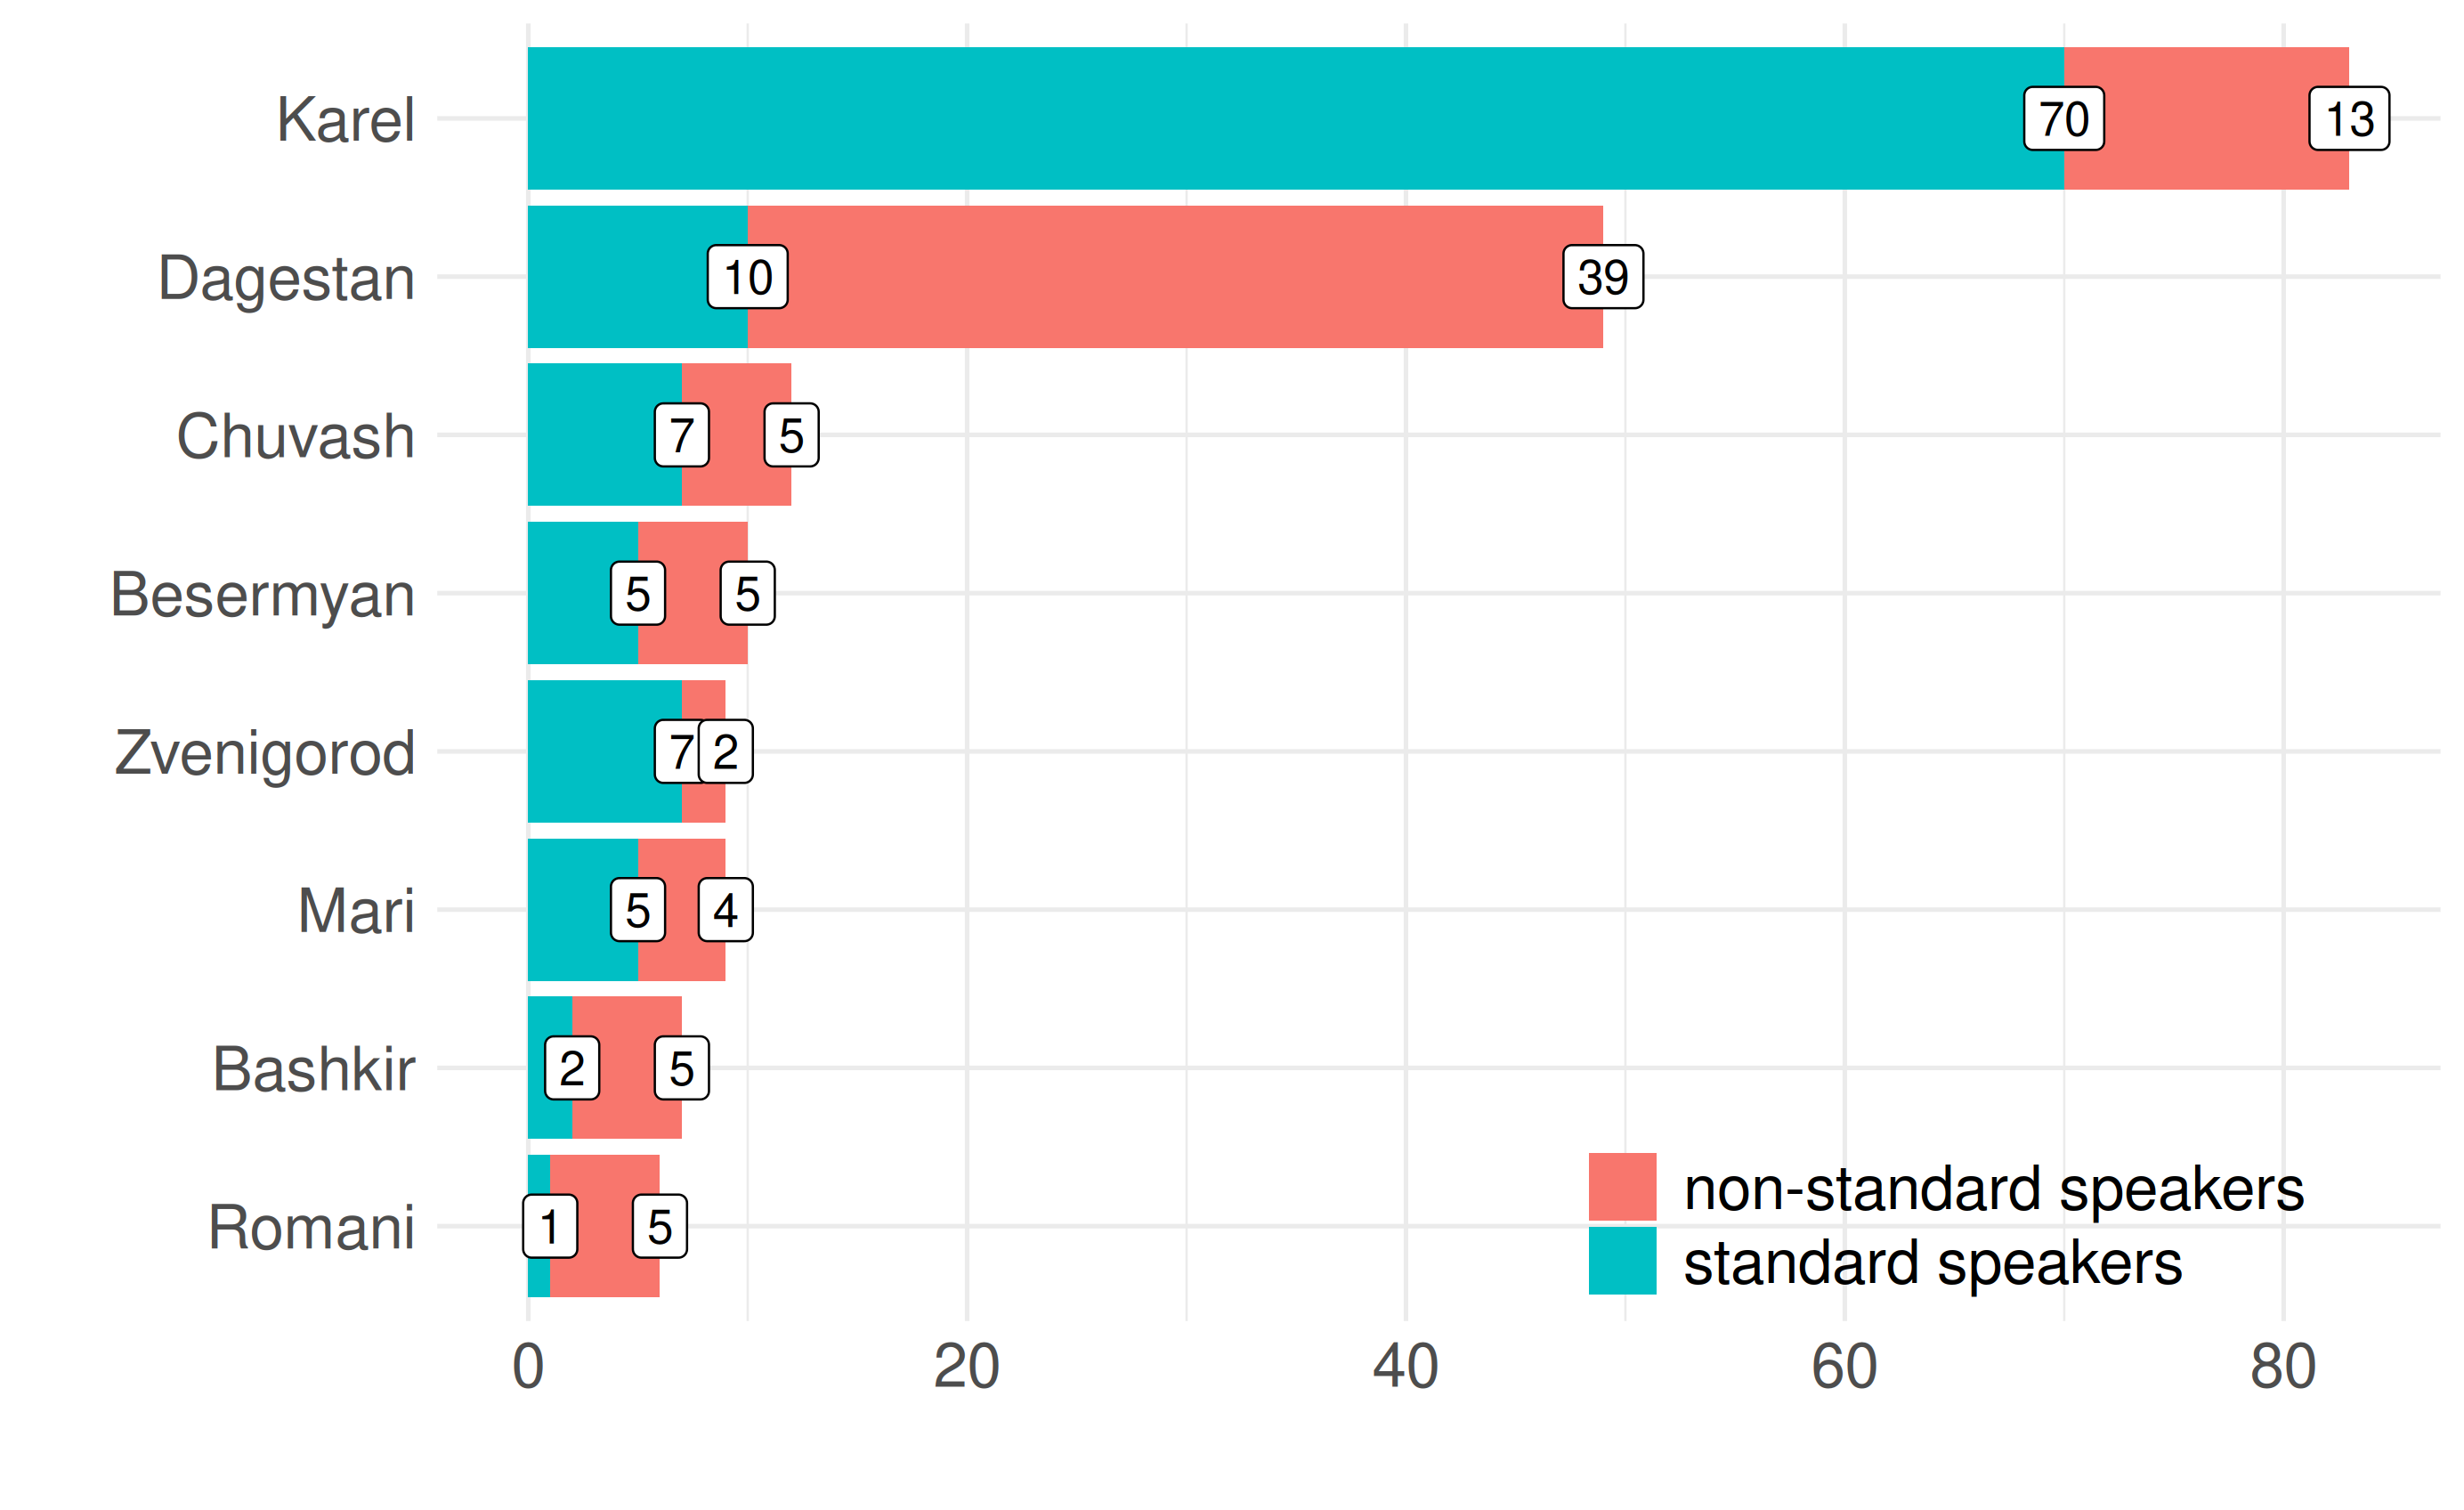
\includegraphics[width=0.93\textwidth,height=\textheight]{images/l2_neg_exist_constr_distribution_of_speakers_by_standardness_across_corpora.png}
\end{center}
\end{frame}

\begin{frame}{Proportion of non-standard occurrences per corpus}
\phantomsection\label{proportion-of-non-standard-occurrences-per-corpus-1}
\end{frame}

\begin{frame}{Types of non-standard marking}
\phantomsection\label{types-of-non-standard-marking}
\begin{itemize}
\tightlist
\item
  Neuter copula

  \begin{itemize}
  \tightlist
  \item
    \emph{gaz ne bylo}
  \end{itemize}
\item
  Non-neuter copula

  \begin{itemize}
  \tightlist
  \item
    \emph{dom\ul{a} ne byl}
  \end{itemize}
\item
  Agreeing subject (could be pattern borrowing for Daghestan)

  \begin{itemize}
  \tightlist
  \item
    \emph{bogatye ljudi ne byli}
  \end{itemize}
\end{itemize}
\end{frame}

\begin{frame}{Statistical modelling}
\phantomsection\label{statistical-modelling-1}
\end{frame}

\begin{frame}{Preliminary conclusions}
\phantomsection\label{preliminary-conclusions}
\begin{itemize}
\tightlist
\item
  Findings comparable to those obtained for NCs
\item
  Variation attested in all L2 corpora, but not to the same extent in
  each of them
\item
  Daghestan as a more uniform variety
\item
  Not all cases of variation can be explained by contact
\end{itemize}
\end{frame}

\section{The DiaL2 sideproject}\label{the-dial2-sideproject}

\begin{frame}{The DiaL2 sideproject}
\phantomsection\label{the-dial2-sideproject-1}
\begin{figure}

\begin{minipage}{0.33\linewidth}

\begin{figure}[H]

{\centering 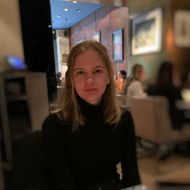
\includegraphics[width=0.63in,height=\textheight]{images/panova.jpeg}

}

\subcaption{Anna Panova}

\end{figure}%

\end{minipage}%
%
\begin{minipage}{0.33\linewidth}

\begin{figure}[H]

{\centering 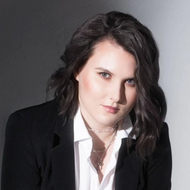
\includegraphics[width=0.63in,height=\textheight]{images/gich.png}

}

\subcaption{Olga Gich}

\end{figure}%

\end{minipage}%
%
\begin{minipage}{0.33\linewidth}

\begin{figure}[H]

{\centering 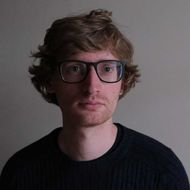
\includegraphics[width=0.63in,height=\textheight]{images/moroz.jpeg}

}

\subcaption{George Moroz}

\end{figure}%

\end{minipage}%

\end{figure}%
\end{frame}

\section{Future plans}\label{future-plans}


\renewcommand\refname{References}
\begin{frame}[allowframebreaks]{References}
  \bibliographytrue
  \bibliography{bibliography.bib}
\end{frame}



\end{document}
